
%DIF LATEXDIFF DIFFERENCE FILE
%DIF DEL EvenDB.tex           Tue Mar 10 12:56:44 2020
%DIF ADD ../Diff/EvenDB.tex   Tue Mar 10 12:50:15 2020

\documentclass[sigplan,10pt]{acmart}
\renewcommand\footnotetextcopyrightpermission[1]{}
\pagestyle{plain}

%========================
%  Packages
%========================
%\usepackage{datetime}
\usepackage{epsfig,subcaption}
\usepackage{url}
%\usepackage{hyperref}
\usepackage{color}
%\usepackage{graphicx}
\usepackage{algorithm}
\usepackage[noend]{algpseudocode}
\usepackage{enumitem}

%========================
%  Macros
%========================

\newcommand{\code}[1]{\textsf{\fontsize{9}{11}\selectfont #1}}

\newcommand{\inred}[1]{{\color{red}{#1}}}
%\newcommand{\inred}[1]{ {#1} } % reddening macro commented out
\newcommand{\remove}[1]{}
\newcommand{\Idit}[1]{\inred{[Idit: #1]}}
\newcommand{\idit}[1]{\inred{[Idit: #1]}}

\newcommand{\sys}{EvenDB}

\newcommand{\tuple}[1]{\ensuremath{\langle \mbox{#1} \rangle}}

\usepackage{cleveref}


\crefformat{section}{\S#2#1#3}


% No date in title area
\date{}

\setlength{\abovecaptionskip}{5pt}
%\setlength{\belowcaptionskip}{0pt}
\setlength{\textfloatsep}{7pt}

% Actual document begins below.
%DIF PREAMBLE EXTENSION ADDED BY LATEXDIFF
%DIF UNDERLINE PREAMBLE %DIF PREAMBLE
\RequirePackage[normalem]{ulem} %DIF PREAMBLE
\RequirePackage{color}\definecolor{RED}{rgb}{1,0,0}\definecolor{BLUE}{rgb}{0,0,1} %DIF PREAMBLE
\providecommand{\DIFadd}[1]{{\protect\color{blue}\uwave{#1}}} %DIF PREAMBLE
\providecommand{\DIFdel}[1]{{\protect\color{red}\sout{#1}}}                      %DIF PREAMBLE
%DIF SAFE PREAMBLE %DIF PREAMBLE
\providecommand{\DIFaddbegin}{} %DIF PREAMBLE
\providecommand{\DIFaddend}{} %DIF PREAMBLE
\providecommand{\DIFdelbegin}{} %DIF PREAMBLE
\providecommand{\DIFdelend}{} %DIF PREAMBLE
%DIF FLOATSAFE PREAMBLE %DIF PREAMBLE
\providecommand{\DIFaddFL}[1]{\DIFadd{#1}} %DIF PREAMBLE
\providecommand{\DIFdelFL}[1]{\DIFdel{#1}} %DIF PREAMBLE
\providecommand{\DIFaddbeginFL}{} %DIF PREAMBLE
\providecommand{\DIFaddendFL}{} %DIF PREAMBLE
\providecommand{\DIFdelbeginFL}{} %DIF PREAMBLE
\providecommand{\DIFdelendFL}{} %DIF PREAMBLE
%DIF END PREAMBLE EXTENSION ADDED BY LATEXDIFF

\begin{document}

\title[\sys: Key-Value Storage for Spatial Locality]{\sys: Optimizing Key-Value Storage\\ for Spatial Locality} 

\author{Eran Gilad}
\affiliation{
\institution{Yahoo Research, Israel} 
}


\author{Edward Bortnikov}
\affiliation{
\institution{Yahoo Research, Israel} 
}

\author{Anastasia Braginsky}
\affiliation{
\institution{Yahoo Research, Israel} 
}


\author{Yonatan Gottesman}
\affiliation{
\institution{Yahoo Research, Israel} 
}


\author{Eshcar Hillel}
\affiliation{
\institution{Yahoo Research, Israel} 
}

\author{Idit Keidar}
\affiliation{
\institution{Technion and Yahoo Research, Israel} 
}

\author{Nurit Moscovici}
\affiliation{
\institution{Outbrain, Israel} 
}

\author{Rana Shahout}
\affiliation{
\institution{Technion, Israel} 
}

\begin{abstract}
Applications of key-value (KV-)storage often exhibit high \emph{spatial locality}, such as  
when many data items have identical composite key prefixes.  
This prevalent access pattern is underused by the ubiquitous LSM  design underlying 
high-throughput KV-stores today.

We present \sys, a general-purpose persistent KV-store optimized for spatially-local %write-intensive
workloads. 
\sys\ combines spatial data partitioning with LSM-like  batch I/O. 
%forgoes the temporal data organization of LSM trees and instead partitions data by key to exploit locality. 
It achieves high throughput, 
ensures consistency under multi-threaded access,   
%offers much faster in-memory access than existing KV-stores, 
and reduces write amplification. 

In experiments with real-world data from a large analytics platform,  \sys\  
%consistently 
outperforms the state-of-the-art. E.g., on a 256GB production dataset, 
\sys\ ingests data $4.4\times$ faster than RocksDB  %scans recently ingested data up to \inred{1.7x} faster, 
and reduces write amplification by nearly $4\times$. 
%\sys\ further outperforms existing solutions whenever the system has sufficient DRAM to hold most of the active working set. 
In traditional YCSB workloads lacking spatial locality, %with working sets that are larger than the available DRAM size, 
\sys\ is on par with RocksDB and significantly better than other open-source solutions we explored.

\end{abstract}

\settopmatter{printfolios=true}
\maketitle

\section{Introduction}
\label{sec:intro}
%%%%%%%%%%%%%%%%%%%%%%%%%%%%%%%%%%%%%%%%%%%%%%%%%%%%%%%%%%%%%%%%%%%%%%%%%
\subsection{Motivation:  spatial locality in KV-storage}
% KV-storage workloads} 
%%%%%%%%%%%%%%%%%%%%%%%%%%%%%%%%%%%%%%%%%%%%%%%%%%%%%%%%%%%%%%%%%%%%%%%%%

% KV-stores are everywhere
Key-value stores (KV-stores) are widely used  by a broad range of applications and are projected
to continue to increase in popularity in years to come; market research  identifies them as the 
``driving factors'' of the NoSQL market, which is expected to garner \$4.2B by 2020~\cite{alliedmarketresearch}.

% In many applications, keys are composite
KV-stores provide a simple programming model. 
Data is an ordered collection of key-value pairs, and the API supports random writes, 
random reads, and range queries. 

A common design pattern is the use of \emph{composite} keys that represent an agglomerate of attributes.
Typically, the primary attribute (key prefix) %-- called the \emph{primary key} -- 
has a skewed distribution, and so   access via the composite key exhibits \emph{spatial locality}, as 
popular key prefixes result in popular key ranges\DIFaddbegin \DIFadd{~\mbox{%DIFAUXCMD
\cite{facebook-workloads}}\hspace{0pt}%DIFAUXCMD
}\DIFaddend . 

One example of this arises in mobile analytics platforms, e.g., AppsFlyer~\cite{appsflyer}, Flurry~\cite{flurry}, 
and Google Firebase~\cite{firebase}. %~\cite{medium-mobile-analytics}.   
Such platforms %help mobile developers collect user activity data, analyze it, and optimize their app experience. They 
ingest massive streams of app event reports %(e.g., start, stop, or particular scenario within an app), 
in  real-time and provide a variety of insight queries into the data. For example, Flurry tracked events from  
1M+ apps across 2.6B user devices  in 2017~\cite{FlurryReport2017}. In order to offer per-app analytics efficiently,
such services aggregate data in KV-stores indexed by a composite key prefixed by a unique app 
id,  followed by a variety of other attributes (time, user id, device model, location, event type, etc.).
%
We examine a trace of almost $2$B  events captured from a production mobile analytics engine 
over half an hour.  
\Cref{fig:cdf} shows the access frequency distribution over the  $60$K app ids occurring in this stream. It follows a marked
heavy-tail pattern: 
%$10$\% of the apps cover over $99.5$\% of the events; 
$1$\% of the apps  cover $94$\% of the events, and fewer 
than $0.1$\% cover $70$\% of them. 

% This means the data is highly skewed and with a very long tail (not depicted in the figure).
%Table~\ref {table:popular} shows the cumulative probability of the top-$20$ popular applications, covering more than $50$\% of the events. 
%With application name as the primary dimension of a composite key this distribution induces high spatial locality.


\begin{figure}[tb]
\centering
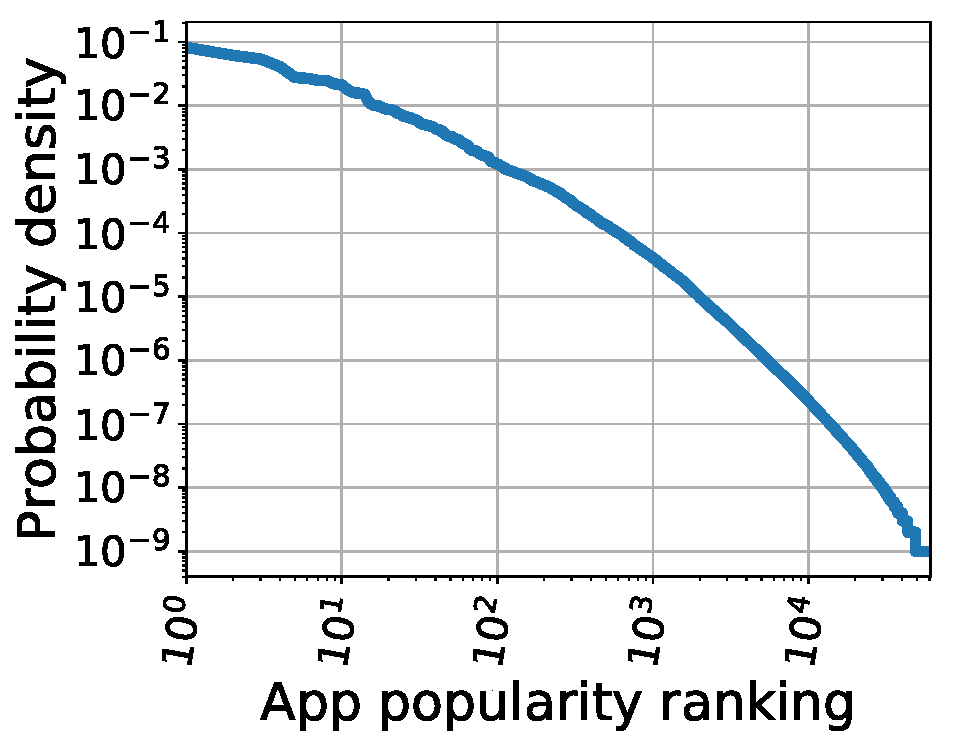
\includegraphics[width=0.6\columnwidth]{figs/app_names_loglog_line.pdf}
\caption{{Distribution of mobile app events by app id (log-log scale) in a production analytics feed (2B events).}}
\label{fig:cdf}
\end{figure}

Composite keys arise in many additional domains, including messaging and social networks\DIFaddbegin \DIFadd{~\mbox{%DIFAUXCMD
\cite{facebook-workloads}}\hspace{0pt}%DIFAUXCMD
}\DIFaddend . 
For example, a backend Facebook Messenger query may retrieve the last 100 messages for a 
given user~\cite{Borthakur:2011:AHG:1989323.1989438}; %, where the primary key is user id. 
in Facebook's social network, a graph edge is indexed by a key consisting of two 
object ids and an association type~\cite{Armstrong:2013:LDB:2463676.2465296}.
%Note further that 
Spatial locality   also arises with simple (non-composite) keys, for example, when 
reverse  URL domains are used as keys for web  indexing~\cite{Cho:1998:ECT:297805.297835}. 

% Overfitting for Zipf 
The prevalence of skewed (e.g., Zipfian)  access  in real workloads is widely-recognized 
and reflected in standard benchmarks (e.g., YCSB~\cite{YCSB}). %  feature heavy-tailed key-access distributions like Zipf.
But these benchmarks fail to capture the spatial aspect of locality, which has gotten far less attention.
% Idit: removed below, too bold
%This, in turn, leads to storage systems being optimized for a skewed distribution on individual keys, % with no spatial locality,
%e.g., in partitioning data by  recent access time as opposed to by key range.
In this work, we make spatial locality a first-class consideration in KV-store design.
% which leads us to rethink the design principles underlying today's popular KV-stores.



%%%%%%%%%%%%%%%%%%%%%%%%%%%%%%%%%%%%%%%%%%%%%%%%%%%%%%%%%%%%%%%%%%%%%%%%%
\subsection{Spatial locality: the challenge}  
\label{ssec:B-tree-compare}
%%%%%%%%%%%%%%%%%%%%%%%%%%%%%%%%%%%%%%%%%%%%%%%%%%%%%%%%%%%%%%%%%%%%%%%%%



% LSM is the standard 
The de facto standard design for high-throughput KV-stores today is \emph{LSM} (log-structured merge) trees~\cite{DBLP:journals/acta/ONeilCGO96}. 
LSMs initially group writes  into files \emph{temporally} rather than by key-range. 
A background \emph{compaction} process later merge-sorts any number of files, grouping data by keys. 

% LSM is  not ideal for spatial locality  because of  temporal grouping 
This approach is not ideal for workloads with high spatial locality for two reasons. 
First,  popular key ranges are fragmented across many files. 
Second,  compaction  is costly in terms of  both performance 
(disk bandwidth) and \emph{write amplification}, namely the number of physical writes 
associated with a single application write. The latter is  particularly important in SSDs as it increases disk wear. 
The temporal grouping means that compaction is indiscriminate with respect to key popularity:  
Since new  files are always merged with old ones, 
 ``cold'' key ranges  continue to be repeatedly re-located by  compactions.  

% LSM is not the best when the entire working set fits in memory
Another shortcoming of LSM is that its temporal organization, while optimizing disk I/O,  penalizes in-memory operation. 
All updates -- including ones of popular keys -- are flushed to disk, even though persistence is assured via a separate \emph{write-ahead-log (WAL)}.
\DIFdelbegin \DIFdel{Beyond increasing write amplification, this makes the flushed keys unavailable for fast read from memory,
which is  wasteful if the system incorporates sufficient DRAM to hold most of the active working set. 
The drop in DRAM prices (more than $6.6$x since 2010~\mbox{%DIFAUXCMD
\cite{dram-prices}}\hspace{0pt}%DIFAUXCMD
) makes the latter scenario increasingly common.  
}\DIFdelend %DIF > Beyond increasing write amplification, this makes the flushed keys unavailable for fast read from memory,
%DIF > which is  wasteful if the system incorporates sufficient DRAM to hold most of the active working set. 
%DIF > The drop in DRAM prices (more than $6.6\times$ since 2010~\cite{dram-prices}) makes the latter scenario increasingly common.  

Yet  LSMs have supplanted the  traditional spatial data partitioning of B-trees for a reason~\cite{rocks-vs-inno}.
%A crucial challenge arising in spatially-organized  storage is how to persist all updates in a consistent way without sacrificing performance.
In  B-trees, each update induces random I/O  to a leaf, resulting in poor write performance.
Moreover, the need to preserve a consistent image of a leaf while it is being over-written induces high write amplification. 
$B^{\epsilon}$-trees~\cite{Brodal:2003:LBE:644108.644201} mitigate this cost using write buffers. % in internal tree nodes. 
However, this slows down lookups, which now have to search in unordered buffers, possibly on disk. 
% If the buffers reside on disk, the lookup time is unacceptably slow, whereas if they are in RAM then they have to be complemented by a separate persistence mechanism, with its own costs.  
%
LSMs, in contrast, achieve high write throughput by absorbing  writes in memory and periodically flushing them as 
sequential files to disk; they expedite reads by caching data in DRAM.

The resounding performance advantage of the LSM approach over B- and B$^{\epsilon}$-trees has been repeatedly demonstrated, 
e.g., in a recent  study of the Percona MySQL server using three storage engines -- RocksDB, TokuDB, and InnoDB --
based on LSM, a B$^{\epsilon}$-tree, and a B-tree, respectively~\cite{toku-rocks-inno}.
%
Another advantage of LSMs is that they readily ensure consistency under multi-threaded access -- in particular, atomic scans --   
via lock-free multi-versioning.
%This can be  tricky when a scan spans both memory-resident and disk-resident data.
In contrast, databases based on B- or  B$^\epsilon$-trees either use locks~\cite{innodblocking} 
or forgo scan consistency~\cite{tucana}.



\remove{
Obviously, we do not claim that spatial data partitioning is new; indeed, classical B-trees~\cite{DBLP:conf/sigmod/BayerM70,Comer79} 
 pre-date  LSM trees, and many B-tree variants~\cite{Brodal:2003:LBE:644108.644201,Bender15, Lehman:1981:ELC:319628.319663} have  emerged over the years. 
 However, it is important to note that these trees are  conceptual constructs rather than storage systems; 
 employing these concepts within a practical data store over a memory hierarchy 
 raises multiple challenges,  which perhaps explains their limited adoption in industrial KV-stores.
 A key challenge is what to persist when and in what format. 
 }

Our  goal is to 
%draw attention to the importance of spatial locality in today's KV-store workloads and to 
put forth a KV-store design alternative  suited for the 
spatial locality arising in today's  workloads, without forfeiting the benefits achieved by the LSM approach.




%%%%%%%%%%%%%%%%%%%%%%%%%%%%%%%%%%%%%%%%%%%%%%%%%%%%%%%%%%%%%%%%%%%%%%%%%
\subsection{Our contribution: \sys}
%%%%%%%%%%%%%%%%%%%%%%%%%%%%%%%%%%%%%%%%%%%%%%%%%%%%%%%%%%%%%%%%%%%%%%%%%

% Drum roll 
We present \sys, a high-throughput persistent KV-store geared towards spatial locality. 
\sys's  architecture (\cref{sec:principles}) combines a spatial data organization with LSM-like  batch I/O. 
The pillars of our design are large \emph{chunks} holding contiguous key ranges. 
\sys's chunks are not merely  a means to organize data on-disk (like nodes in a B-tree). They 
are also the basic units for read-write DRAM caching, I/O-batching, logging, and compaction. 
This approach is unique.
%Typical KV-stores rely on OS-managed page caches (whereas chunks consist of many pages)  
%supplemented by application-level caches. 
Typical KV-stores rely on finer-grain OS- and application-level page caches (whereas chunks consist of many pages) and employ a global WAL. 

\remove{
B-trees, e.g., InnoDB, use read-write page caches~\cite{InnoDB-Buffer-Pool}, however they fail to capture spatial locality 
because their cache granularity is too fine, which results in poor-performing near-random writes~\cite{toku-rocks-inno}.  
LSM's, e.g., RocksDB, use caches for the read path only~\cite{RocksDB-blockcache}. Their temporal structure optimizes write
performance in the short term but degrades it in the long term, due to compactions. Here too, 
spatial locality remains unexploited.}

Our novel chunk-based organization has several benefits. 
First, chunk caching is effective for spatially-local workloads.
Second, chunk-level logging eliminates the need to log each update in a system-level WAL, thus 
reducing write amplification and expediting crash-recovery. 
Finally, using the same data structure for both the read-path (as a cache) and the write-path
(as a log) allows us to perform \emph{in-memory compaction}, reducing write amplification even further.

% Downsides
The downside of spatial partitioning is that if the data lacks spatial locality and the active working set is big, 
chunk-level I/O batching is ineffective. Moreover, 
caching an entire chunk for a single popular key is wasteful. 
We mitigate the latter by adding a \emph{row cache} for read access to hot keys. Even so, 
our design is less optimal for mixed read/write workloads lacking spatial locality, for which the LSM approach may yield better performance.  

%To further expedite access in different scenarios, we incorporate a number of additional mechanisms: 
%a volatile index for direct access to chunks by key; Bloom filters to reduce reads from disk-resident chunks; and 

Our algorithm (\cref{sec:design}) is designed for high concurrency. 
%among threads running put, get, and scan operations, as well as background maintenance (compaction). 
It supports atomic scans using low-overhead multi-versioning, where versions are increased only by scans and not by updates. 
It ensures consistency and correct failure-recovery. 
%While the mechanisms we employ are all variants of ones appearing in the literature, their combination is novel and results in a high-performance storage system.

We implement \sys\ in  C++ (\cref{sec:impl}) and extensively evaluate it (\cref{sec:eval})
via three types of workloads: (1) a production trace collected from a large-scale mobile analytics platform; 
(2)  workloads with synthetically-generated composite keys exercising  standard YCSB scenarios~\cite{YCSB};
and (3)  YCSB's traditional benchmarks, which employ simple (non-composite) keys.  
%In all cases, 
We compare \sys\ to the recent (Oct 2018) release of RocksDB~\cite{RocksDB}, a mature industry-leading LSM KV-store. 
We  experimented with two additional open-source KV-stores, PebblesDB~\cite{PebblesDB}  and  
% PreconaFT/
TokuDB~\cite{TokuDB} (the only publicly-available $B^{\epsilon}$-tree-based 
KV-store); both performed significantly worse than  RocksDB and \sys, so we focus on RocksDB results. 
%so we do not discuss them further.
%\inred{across the entire YCSB benchmark suite.} %, which is in line with previous studies of PerconaFT~\cite{tucana}, so we excluded them from further tests. 
Our main findings are: 
\begin{enumerate} 
  %   \setlength{\itemindent}{-10pt}
\item \sys\/ is  better than RocksDB under high spatial  locality.  
For instance, on a 256GB production dataset, \sys\ ingests data \DIFdelbegin \DIFdel{4.4x }\DIFdelend \DIFaddbegin \DIFadd{$4.4\times$ }\DIFaddend faster than RocksDB %,  scans recent  data up to 27\% faster, 
and reduces write amplification by almost \DIFdelbegin \DIFdel{4x}\DIFdelend \DIFaddbegin \DIFadd{$4\times$}\DIFaddend . 
%And in large synthetic composite-key workloads, \sys\  improves over RocksDB's throughput by $24\% - 75\%$. 
\item \sys\/ significantly outperforms RocksDB whenever most of the working set fits in RAM, 
%For example, with synthetic composite keys and a memory-resident working set, \sys\  
accelerating scans by up to \DIFdelbegin \DIFdel{$3.5$x}\DIFdelend \DIFaddbegin \DIFadd{$3.5\times$}\DIFaddend , puts by up to \DIFdelbegin \DIFdel{$2.3$x}\DIFdelend \DIFaddbegin \DIFadd{$2.3\times$}\DIFaddend , and gets by up to \DIFdelbegin \DIFdel{$2$x}\DIFdelend \DIFaddbegin \DIFadd{$2\times$}\DIFaddend . 
\item \sys's performance is  comparable to RocksDB's in traditional YCSB workloads without spatial locality.
%while its write amplification is much smaller.
\item RocksDB outperforms \sys\ (by 20--25\%)  in mixed read/write workloads with large active working sets and no spatial locality, 
although \sys's write amplification remains \DIFdelbegin \DIFdel{$\sim$2x }\DIFdelend \DIFaddbegin \DIFadd{$\sim2\times$ }\DIFaddend smaller than RocksDB's. 
%\item \sys\ has lower write amplification, especially on large datasets.
\end{enumerate}

% Benefits
Our results underscore the advantages of \sys's spatially-organized chunks:
(1) eliminating fragmentation of key ranges  yields better  performance under spatial locality; 
(2) keeping hot ranges in memory leads to better performance when most of the working set fits in RAM; and 
(3) in-memory chunk compaction saves disk flushes and reduces write volume.  
In addition, in-chunk logging allows quick recovery from crashes with no need to replay a WAL.


~\cref{sec:related}  surveys related work and~\cref{sec:conclusions} concludes this paper. 


\section{Design Principles}
\label{sec:principles}

\subsection{Access semantics and optimization goals}
\sys\ is a persistent ordered key-value store. Similarly to popular industrial ones~\cite{hbase,leveldb,RocksDB}, 
it supports concurrent access by multiple threads and ensures strong consistency. 
Specifically its \emph{put, get}, and \emph{scan} operations are \emph{atomic}.  
For scans, this means that all key-value pairs returned by a single scan belong to a consistent 
snapshot reflecting the state of the data store at a unique point in time.

\sys\ persists data to disk to allow it to survive crashes.
%Following a crash, \sys\ recovers to a consistent state reflecting an execution point before the crash.
As in other systems~\cite{leveldb,RocksDB},  it supports
\emph{asynchronous} persistence, where puts are buffered before being persisted in the background,  
 trading durability for speed. In this case, some recent updates may be lost but 
 recovery is to a \emph{consistent} state  in the sense that 
if some put is lost, then no ensuing (and thus possibly dependent) puts are reflected.



Our key optimization goals are the following:
\begin{enumerate}
%\itemsep0pt
\item Optimize for {spatial locality}, e.g., workloads that employ composite keys.
\remove{
 Many NoSQL applications embed multi-dimensional data in a single-dimension composite key. 
 This design provides high spatial locality on the primary dimension (key prefix). We strive
 to express this locality in physical data organization.
 }

\item Minimize {write amplification}  to reduce disk wear.%, especially for SSD devices.

\item %{\bf High performance  with memory-resident working sets.}
%To sustain high speed, key-value stores nowadays leverage increasing RAM sizes where they can hold most of the active working set. 
Strive for high performance in  \emph{sliding-local} scenarios, where most of the active working set fits in DRAM. 
Note that we do \emph{not} expect the entire database to fit in
memory, only the active data.  

\item Ensure {fast recovery} to a consistent state.  
%Because crashes are inevitable, recovery must ensure consistency and the downtime it entails should be kept  short. 
\end{enumerate}

\subsection{Design choices}

\sys\ combines the spatial \DIFdelbegin \DIFdel{locality }\DIFdelend \DIFaddbegin \DIFadd{data partitioning }\DIFaddend of B-trees with the optimized I/O and quick access of LSMs. 
Its data layout is illustrated in Figure~\ref{fig:piwi}.  We now discuss its key components.   

\begin{figure}[tb]
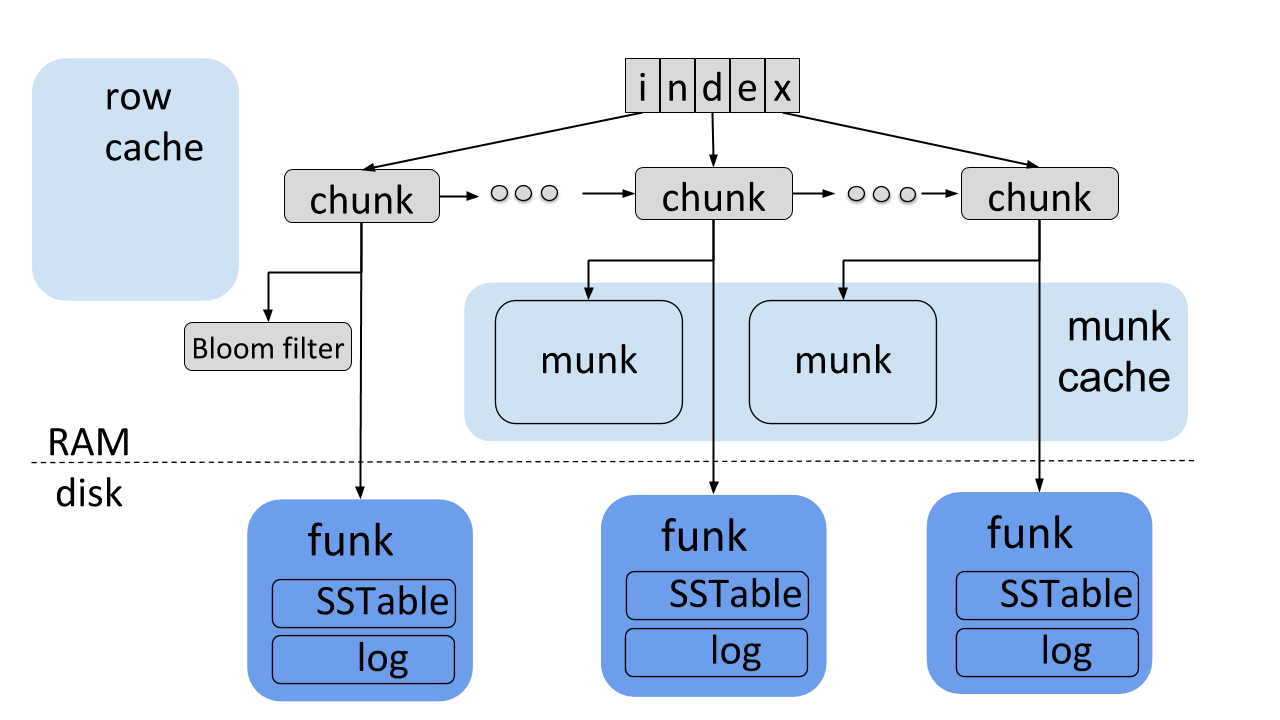
\includegraphics[width=\columnwidth]{PiWi.png}
\caption{\sys's  organization. Gray boxes depict metadata, light blue areas show RAM caches of KV-pairs, and blue areas represent on-disk KV storage.}
\label{fig:piwi}
\end{figure}


{\bf Chunks.\ }
To leverage spatial locality, we partition data -- both on-disk and in-memory -- by key.
Our  data structure is organized as a 
%sorted linked 
list of \emph{chunks} holding consecutive key ranges. 
All chunks are represented in memory via lightweight volatile metadata objects, which are reconstructed from disk on recovery.

{\bf Sequential I/O with in-chunk logging.\ }
For persistence, each chunk has a file representation called  \emph{funk} (file chunk), which holds all the KV-pairs in the chunk's range.
Within funks, we adopt LSM's sequential I/O approach. To this end, the funk 
is divided into two parts: (1) a sorted \emph{SSTable} (Sorted String Table~\cite{Bigtable2008}), and (2) an unsorted \emph{log}. 
New updates are appended to the log; the log is  merged into the SSTable via an infrequent background compaction process. 
Under spatial locality,  popular chunks are targeted frequently, allowing effective batching of their log updates. 
Unlike LSMs, \sys\ logs writes exclusively within their funks and avoids duplicating the updates  in a separate WAL. This reduces write amplification and expedites recovery. 

{\bf Chunk-level caching with in-memory compaction.\ }
DRAM caches are instrumental for read performance. 
To favor workloads with spatial locality, we cache entire chunks:
a popular chunk is cached in a  memory data structure called \emph{munk} (memory chunk).
Like their on-disk counterparts, munks have a compacted sorted prefix while new updates are appended at the end and remain unsorted until the next compaction. 
Whereas LSM caches  only serve the read-path, caching at the chunk granularity allows us to 
leverage munks also in the write-path, specifically, for in-memory compaction.  
We observe that 
%Whereas appending writes to the log is essential for persistence, 
compacting a funk's log is only required for performance (to expedite on-disk lookup) and is redundant whenever the chunk is cached. Thus, when 
a chunk has a munk, we compact it almost exclusively in memory and allow the disk log to grow. 
Note that if a chunk does not have a munk, it usually means that the chunk is ``cold'' 
and hence there is little or no new data to compact. So either way,  disk compaction is rare, and write amplification is low.

{\bf Fast in-memory access.\ }
Chunks are organized in a sorted linked list. To speed up lookups, they are indexed using a volatile index (a sorted array in our implementation).  

 
 {\bf Row caches and Bloom filters.\ }
 \sys\ adopts two standard mechanisms from LSMs. First, to expedite access to  keys whose chunks are only on-disk  (i.e., have no munks), 
a \emph{row cache} of individual popular keys serves the read-path. The row cache is important for workloads that lack
spatial locality where caching an entire chunk for a single ``hot'' key is wasteful. 
Second, for munk-less chunks, we employ \emph{Bloom filters} to limit excessive access to disk. 
\DIFaddbegin \DIFadd{The Bloom filter is maintained as long as the chunk has no munk, and is re-created whenever a munk is evicted.
}\DIFaddend 

{\bf Concurrency and multi-versioning.\ }
 \sys\ allows high parallelism among threads invoking its API calls. 
 Get operations are wait-free (never block) and puts use lightweight synchronization. 
 To support atomic scans, we  employ a light form of multi-versioning that uses 
copy-on-write to keep old versions only if they may be required by ongoing scans. 
In other words, if a put attempts to overwrite a key required by an active scan, then a new version is created alongside the 
existing one, whereas versions that are not needed by any scan are not retained. 
Version management incurs a low overhead because it occurs only on scans. 
%It also defines a simple rule for garbage collecting old versions.
In addition, tagging each value with a version allows \sys\ to easily recover to a consistent point in time, namely a version below which all puts have been persisted to disk.



\section{\sys's Design}
\label{sec:design}


In~\cref{ssec:layout} we present \sys's data organization. 
We discuss concurrency control and atomic scans in~\cref{ssec:scans}.
\cref{ssec:ops} overviews \sys's normal %(maintenance-free) 
operation flow, while   the data structure's maintenance is discussed in~\cref{ssec:rebalance}.
Finally,~\cref{ssec:flush-recovery} discusses data flushes and failure recovery.


\subsection{Data organization}
\label{ssec:layout}

% \paragraph{Chunks, funks, and munks.}

\sys's data layout is depicted in Figure~\ref{fig:piwi}.
Data is partitioned into chunks, each holding a contiguous key range.
Each chunk's data 
(keys in its range and their corresponding values) 
is kept on-disk (funks, for persistence), and possibly in-memory (munks, for fast access). 
Munks can be replaced and loaded from funks at any time based on an arbitrary replacement policy.
Chunk metadata objects are significantly smaller than munks and funks
(typically, less than 1 KB vs. tens of MBs) and are always kept in memory.

A volatile \emph{index} maps keys to chunks. 
Index updates are lazy, offering only best-effort expedited search.

A funk consists of two files:  a compacted and sorted KV map \emph{SSTable} %(Sorted String Table~\cite{Bigtable2008}) 
and a write \emph{log}. When a funk is created, the {former} holds all the chunk's KV pairs and the {latter}  is empty.
New KV pairs are subsequently appended to the  {log}. If a key is over-written, its old value remains in the {SSTable} while the new one  is added to the {log} (the {log} is more up-to-date).

\remove{
\begin{figure}[tb]
\centerline{
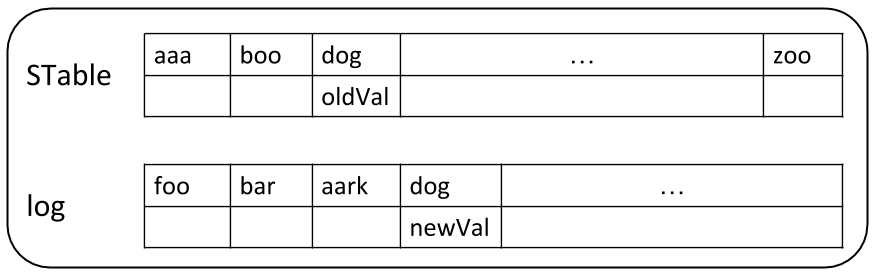
\includegraphics[width=0.75\columnwidth]{funk.png}
}
\caption{A \sys\ funk consists of a sorted {SSTable} and an unsorted {log} holding the most recent updates.}
\label{fig:funk}
\end{figure}
}

This structure allows us to benefit from sorted searches on the {SSTable} and at the same time
to update chunks without relocating existing data, thus minimizing write amplification.
As a funk's {log}  grows, however, searching becomes inefficient   and  
the funk is no longer compact, i.e., it may contain redundant (over-written) values.
Therefore, once the {log}  exceeds a certain threshold, we reorganize the funk
via a process we call \emph{rebalance}, as explained below.
\DIFaddbegin \DIFadd{The rebalance threshold controls the system's }\emph{\DIFadd{write amplification}}\DIFadd{, namely, the additional space consumed on top of the raw data.
Note that the additional space amplification induced by fragmentation is negligible, because chunks typically consist of $\sim$1000 pages.
}\DIFaddend 

% Thus, multiple \emph{generations} of munks may exist for a chunk throughout its life time.
%Chunks that are not cached are denoted \emph{munk-less}.
%The details of the chunk's metadata structure are deferred to the the supplemental material.

A munk holds KV pairs in an array-based linked list.  
\remove{
A munk consists of two arrays -- \emph{karray} for keys and \emph{varray} for values. The  \code{karray}  holds a sorted linked list of the chunk's keys
with pointers to values in the \code{varray}. 
}
When a munk is created, some prefix of this array is populated,
sorted by key, so each cell's successor in the linked list is the ensuing cell in the array.
New KV entries are appended after this prefix.
As new entries are added, they create bypasses in the linked list, and consecutive keys in the
list are no longer necessarily adjacent in the array. Nevertheless, as long as 
a sizable prefix of the  array  is sorted and insertion order is random, bypasses are short in expectation.
\remove{Key removals, in turn, leave obsolete values in the munk, so it is no longer compacted.}
Keys can thus be searched efficiently via binary search on the sorted prefix followed by a short traversal 
of a bypass path. % at the suffix of the array. 
%This approach was previously used in in-memory data structures, e.g., Kiwi~\cite{kiwi}.  

As KV pairs are added, overwritten, and removed, munks and funks need to undergo reorganization. This includes  
(1) \emph{compaction} to garbage-collect removed and overwritten data, 
(2) \emph{sorting} keys to make searches more efficient,  and
(3) \emph{splitting} overflowing chunks.
Reorganization is performed by three procedures: 
(1) Munk rebalance (creating a new compacted and sorted munk instead of an existing one) 
happens in-memory, independently of disk flushes. 
(2) Funk rebalance (on-disk) happens much less frequently. 
(3) Splits  create new chunks as well as new  funks and munks.

%\paragraph{Expediting reads.}

Whenever a chunk is cached (i.e., has a munk), access to this chunk is particularly fast:
the chunk metadata is quickly located using the index, the munk's sorted prefix allows for fast 
binary search, and updates are added at the end of the munk's array and appended to the funk's log.
% Thus, \sys\ is particularly fast when almost the entire working set is memory-resident. 
We take two measures to mitigate the performance penalty of accessing keys in non-cached chunks.

First, we keep a row cache holding popular KV pairs only from munk-less chunks. Note that unlike munks, which cache key ranges, the row
cache holds individual keys, and is thus more effective in dealing with point queries (gets as opposed to scans) with no
spatial locality.

If the active working set is larger than the available DRAM, these two caches might not suffice, and so a certain portion of reads 
will be served from disk. Here, the slowest step is the sequential search of the {log}. 
To reduce such searches, a chunk with no munk holds a Bloom filter for the corresponding funk's {log}, 
which eliminates most of the redundant log searches.
The Bloom filter is partitioned into a  handful of filters, each summarizing the 
content of part of the {log}, limiting  sequential  searches to a small section of the log.

 

 \subsection{Concurrency and atomic scans}
\label{ssec:scans}

\remove{
\paragraph{Chunk metadata structure.}

The metadata structure is given in Algorithm~\ref{alg:chunk}. 
The first field is its \code{state}, which is explained in \cref{ssec:rebalance}  below. 
It next holds a pointer to the appropriate funk, and either a munk or a Bloom filter, as well as a pointer to the next 
chunk in the chunk linked list.
\remove{
It further keeps the generation number of its latest munk, \code{gen}, and a per-generation sequence number,
\code{seq}, which, in case there is an active munk, is the index of the next free cell in the munk's  \code{karray}  and \code{varray}. The chunk's \code{gen} and \code{seq} are stored together in one 64-bit word to allow 
atomic access to both of them. 
}
%It further includes a Bloom filter as explained above.
Finally, the chunk includes locks to synchronize concurrent access by multiple threads, as explained below.

\begin{algorithm}[htb]

\begin{algorithmic}
\State \code{state} \Comment  baby, child, active, asleep, or aged
\State ptr \code{funk} \Comment funk disk address
\State ptr \code{munk} \Comment munk memory pointer
\State ptr \code{next} \Comment next chunk in linked list
%\State int \code{gen} \Comment munk generation
%\State int \code{seq} \Comment sequence number in current generation 
\State ptr \code{bloomFilter} \Comment summary of set of keys in \code{log}
\State asymmetric lock \code{rebalanceLock} \Comment shared/exclusive lock 
\State lock \code{funkChangeLock} \Comment acquired with try\_lock 
% \State \code{$\langle$key, version, done, counter$\rangle$  PPA[threads]} \Comment pending puts
\end{algorithmic}

\caption{Chunk metadata structure.}
\label{alg:chunk}
\end{algorithm}
}

%\paragraph{Thread synchronization variables.}

\sys\ allows arbitrary concurrency among operations. Gets are wait-free and proceed without synchronization. 
In order for scans to be atomic, they synchronize with puts, potentially waiting for some puts to complete
(puts never wait for scans). Puts also synchronize with rebalance operations. 
% (invoked in background threads). 

\remove{
We note that using a single pending array to synchronize all operations can cause contention, which we
eliminate in our implementation by tracking the pending puts in per-chunk arrays with per-thread entries as done in~\cite{kiwi}.
}

To support atomic scans we employ a system-wide \emph{global version (GV)}. 
A scan  creates a \emph{snapshot} associated with GV's current value by fetching and incrementing GV.
This signals to ensuing put operations that they must not overwrite the highest
version smaller than the new GV value.
This resembles a \emph{copy-on-write} approach, which  creates a virtual snapshot by 
indicating that data pertaining to the snapshot should not be overwritten in-place.  

To allow garbage collection of old versions, \sys\  tracks the snapshot times of active scans.
This is done in a dedicated  \emph{Pending Operations (PO)} array, which has one entry per active thread,
and is also used to synchronize puts with scans as explained shortly.
The compaction process 
%that runs as part of rebalance 
removes old versions that are no longer required for any  
scan listed in PO. Specifically, for each key, it removes versions older than the highest version smaller than the minimal
scan entry in PO and the value of GV when the rebalance begins. 

\remove{
For linearizing (i.e., determining an order on) updates, we associate each KV pair written to the data store 
with a unique-per-key timestamp.
This timestamp is composed as a tuple $\langle$ver, gen, seq$\rangle$, where \emph{ver} is  the version read from GV 
(recall that GV is only incremented upon scans and hence might remain unchanged across multiple puts),
\emph{gen} is the generation of the target chunk's last created munk  (which may or may not still exist), 
and seq is the running sequence number of values inserted to the chunk in the current generation.
}

% \paragraph{Concurrent puts and scans.}

A put obtains a version number from GV without incrementing it. Thus, multiple puts may write values with the same version, each over-writing the previous one. 
%Ordering concurrent puts with the same key and version is discussed in the next section where we elaborate on the put operation's logic.

%A scan begins by fetching-and-incrementing GV.
If a put obtains its version before a scan increments GV, the new value must be included in the scan's snapshot. 
However, because the put's access to the GV and the insertion of the new value to the chunk do not occur atomically,
a subtle race may arise. Assume a put obtains version $7$ from GV and then stalls before
inserting the value to the chunk while a scan obtains version $7$ and increments GV to $8$. If the scan proceeds 
to read the affected chunk, it misses the new value it should have included in its snapshot.
%
To remedy this, puts announce (in PO) the key they intend to change when beginning their operations and scans wait for relevant pending puts to complete; see the next section for details.
%This mechanism is a simplification of the non-blocking put-scan synchronization employed (and proven correct) in~\cite{kiwi}.

%For symmetry, get operations synchronize with puts the same way that scans do. 

\remove{
A put operation takes hold of the chunk's \code{rebalanceLock} in shared mode, 
then publishes itself in  PO, gets a version by reading GV, updates its version in PO,  
and releases the chunk lock. 
}


\remove{
% Simplified PPA
  The per-chunk PPA is used to synchronize pending puts  with ongoing scans. It holds an entry for every active inserting thread, consisting of a \code{key},  a \code{version}, 
 a \code{done} bit indicating whether the update has been completed, and a monotonically increasing 
 \code{counter} to avoid ABA scenarios.

A put operation first registers itself in the appropriate chunk's PPA entry with the key it intends to put.
It then reads GV and sets the version field in its PPA entry to the read version. 
After completing the actual put (in the appropriate munk and/or funk), it sets the \code{done} bit.
A scan, in turn, scans the PPA in addition to the chunk's data 
(\code{karray},  \code{log} or \code{SSTable}  ). If it finds a pending put
of a relevant key that is not yet associated with a version, it waits for the version to be assigned. 
Once the version is assigned, if it is the highest version for this key that does not exceed its scan time, 
it waits for the \code{done} bit to be true or for the the \code{version} to change again, at  which point
it reads the value from the appropriate munk or funk.
}

Rebalance operations synchronize with concurrent puts using the chunk's \emph{rebalanceLock}.
This is a shared/exclusive lock, acquired in shared mode by puts and in exclusive mode (for short time periods)
by rebalance. 
%, which is held for short time periods during chunk, funk, and munk replacements.  
Gets and scans do not acquire the lock. Note that it is safe for them to read from a chunk while it is being replaced because
(1) rebalance makes the new chunk accessible only after it is populated, and (2) a chunk is immutable during rebalance, so 
the newly created chunk holds the same content as the displaced one.

To minimize I/O, we allow at most one thread to rebalance a funk at a given time. This is controlled by 
the  \emph{funkChangeLock}, which is held by the thread rebuilding the  chunk. 
It is acquired using a try\_lock, where threads that fail to acquire it do not retry but instead wait for the winning thread to complete the funk's creation.

\subsection{\sys\ operations}
\label{ssec:ops}

\Cref{alg:ops}  presents pseudocode for \sys's operations. 
Both get and put begin by locating the target chunk using the \code{lookup} function. In principle, this can be done by traversing the chunk list, but that would result in linear search time. To expedite the search,   \code{lookup} first searches the index. But because index updates are lazy -- they occur after the new chunk is already
in the linked list --  the index may return a stale chunk that had already been replaced by rebalance. To this end, the index search is repeated with a smaller key in case the index returns a stale chunk, and the index search is supplemented by a linked-list traversal. 
%A similar approach was used in earlier works~\cite{kiwi,tdls}. 


\begin{algorithm}[tb]
\begin{algorithmic}[1]{}
\Procedure{get}{key}	
		\State $C \leftarrow$ \code{lookup(key)}

%		\State $T \leftarrow  \{ \langle \code{th}, i \rangle : \code{C.PPA[th].key = key }  $ 
%		\Statex \hspace{21mm}	$ \wedge \; \code{C.PPA[th].counter} = i \}$ 



%		\code{th} $\in T$,  
%		\Statex  \hspace{21mm}		$C.$\code{PPA[th].done} $\vee$ \code{$C$.PPA[th].ver $>$ gv}
		\If{$C$.\code{munk}} 
			\State search \code{key} in $C$.\code{munk} linked list;  return 
		\EndIf
		\State search \code{key} in row cache; return  if found
		\If{\code{key}$\in C.$\code{bloomFilter}}  
			\State	search \code{key} in \code{funk.log}; return  if found
		\EndIf
		\State	search \code{key} in \code{funk.SSTable}; return  if found
		\State return NULL	
\EndProcedure
\Statex
\Procedure{put}{key, val}	
		\State $C \leftarrow$ \code{lookup(key)}
		\State lockShared($C$.\code{rebalanceLock})
		\State  \code{PO[i]}  $\leftarrow$ \code{$\langle$put, key, $\bot \rangle$ }
			 \Comment publish  thread's presence 
		\State \code{gv} $\leftarrow$ \code{GV}   \Comment read global version
		\State  \code{PO[i]}  $\leftarrow$ \code{$\langle$put, key, gv$\rangle$ }
			\Comment write version in \code{PO}
%		\Statex \Comment atomically allocate entry in munk and get its pointer
%		\State \code{$\langle$gen, seq$\rangle$ } $\leftarrow$ F\&I ($C$.\code{$\langle$gen, seq$\rangle$})
%		\State \code{munk} $\leftarrow$ $C$.\code{munk} \Comment read atomically with \code{gen}
		\Statex \Comment write  to funk log, munk (if exists), and row cache  
		\State append \code{$\langle$key, val, gv$\rangle$} to \code{funk.log}
		\If{$C$.\code{munk}} 
			\State add  \code{$\langle$key, val, gv$\rangle$} to $C$.\code{munk}'s linked list
%			\State \code{munk.karray[seq]}  $\leftarrow$ \code{key}
%			\State \code{munk.varray[seq]}  $\leftarrow$ \code{val}
%			\State link \code{munk.karray[seq]} into   \code{munk.karray}
		\Else \Comment no munk -- key may be in row cache
		\State update \code{$\langle$key, val$\rangle$} in row cache (if key is present)
		\EndIf
		\State unlock($C$.\code{rebalanceLock})
		\State \code{PO[i]}  $\leftarrow \bot$ \Comment put is no longer pending
\EndProcedure
\Statex
\Procedure{scan}{key1, key2}
		\State  \code{PO[i]}  $\leftarrow$ \code{$\langle$scan, key1, key2, $\bot \rangle$ } \Comment publish scan's intent 
		\State \code{gv} $\leftarrow$ \code{F\&I(GV)}   \Comment fetch and increment global version
		\State  \code{PO[i]}  $\leftarrow$ \code{$\langle$scan, key1, key2, gv$\rangle$ }
		\Comment publish version in PO
		\State  $T \leftarrow $  PO entries updating keys in range [\code{key1, key2}] 
		\State wait until $\forall t \in T, t$  completes or has a version $>$   \code{gv}
		\State $C \leftarrow$ \code{lookup(key1)}
		\Repeat
%			\If{$C$.\code{munk}} 
				\State collect from $C$.\code{munk} or $C$.\code{funk} (log and SSTable)
				\Statex \hspace{1cm} max version $\le$\code{gv} for all keys in [\code{key1, key2}] 

%			\Else
%				\State get max version $\le$\code{gv} for keys in $C$.\code{funk}
%			\EndIf
			\State $C \leftarrow C$.\code{next} 
		\Until{reached \code{key2}}
%		\State return collected values
\EndProcedure	
\end{algorithmic}
\caption{\sys\ normal operation flow for thread \code{i}.}
\label{alg:ops}
\end{algorithm}



\paragraph{Get.}
%{Gets} proceed without synchronization. 
If the chunk has a munk, {get} searches the key in it by first running a binary search on its sorted prefix and then traversing linked list edges as needed. 
Otherwise,  {get} looks for the key in the {row cache}. If not found, it queries 
the {Bloom filter} to determine if the key might be present in the target chunk's  
 {log}, and if so, searches for it there.  If the key is in none of the above, the {SSTable} is searched.

\remove{
A {put} proceeds by allocating the next free entry in 
the munk to its value by atomically fetching-and-incrementing the chunk's 
$\langle$ \code{gen}, \code{seq} $\rangle$ pair. It obtains the \code{munk} atomically with 
the read of \code{gen} in order to ensure that \code{seq} indexes the correct array. 
This can be done by re-reading  \code{gen} or by loading one object that references both.
} 

\paragraph{Put.}
Upon locating the chunk,  {put} grabs its {rebalanceLock} in shared mode to ensure that it is not being rebalanced.
% during the {put} operation. 
It then registers itself in PO with the key it intends to put,
reads GV, and sets the version field in its PO entry to the read version. 
The {put} then proceeds to write the new KV pair to the  funk's {log} and to the 
munk, if exists. 
If the funk has no munk and the row cache contains an old value of the key, the row cache is then updated.
The munk and funk are multi-versioned to support atomic scans, 
whereas the row cache is not used by scans and holds only the latest version of each key. 
%In case the put's version is the same as the current latest one, it over-writes the current one in the munk but appends a new one in the funk's log. 
Finally, a put unregisters itself from PO, indicating completion, and releases the chunk's rebalance lock.

We note that in case multiple puts concurrently update the same key with the same version, they
may update the funk and munk (or the funk and row cache) in  different orders,
and so the latest update to one will not coincide with the latest update to the other. 
This can be addressed, for example, by locking keys. 
Instead, we opt to use a per-chunk monotonically increasing counter (not shown in the code) to determine 
the order of concurrent put operations updating the same key with the same version. % (similarly to~\cite{kiwi}).
We  enforce updates to occur in order of version-counter pairs by writing them alongside the values in the munk, 
PO, funk, and row cache.
Following a split, the new chunks inherit the counter from the one they replace.  


\paragraph{Scan.}
A scan first publishes its intent to obtain a version in PO, to 
signal to concurrent rebalances not to remove the versions it needs. It
fetches-and-increments GV to record its snapshot time \code{gv},  
and then publishes its key-range and \code{gv} in PO.
Next, the scan waits for the completion of all pending puts  
that might affect it  -- these are puts of keys in the scanned key range that either do not have a version yet or have versions lower than the scan time.
This is done by busy waiting on the PO entry until it changes; monotonically increasing counters are used 
in order to avoid ABA races. 

Then it collects the relevant values from all chunks in the scanned range.
Specifically, if the chunk has a munk, the scan reads from it, for each key in its range, 
the latest version of the value that precedes its snapshot time.
Otherwise, the scan collects all the relevant versions for keys in its range from both 
the {SSTable}   and the {log} and merges the results.
Finally, the scan unregisters from PO.
 %are executed by calling \code{createSnapshot(fromKey, toKey)} 
%and then iterating over the key range with \code{next} calls.

\subsection{Rebalance}
\label{ssec:rebalance}

Munk (resp.\ funk) rebalance improves the data organization in a munk (funk) by removing old versions that are no longer needed 
for scans, removing deleted items, and sorting all the keys. It is typically triggered when the munk (funk) exceeds a capacity threshold.   
The threshold for funk rebalance is higher when it has a munk, causing most rebalances to occur in-memory.
%It can be triggered either by a thread attempting to access the chunk or a dedicated background thread.
%In case a chunk has a munk, rebalance reorganizes only the munk, since all searches are served by it. 
%The respective funk is reorganized much less frequently, merely in order to bound the log's growth. 
Rebalance creates  a new munk (funk) rather than reorganize it in-place 
in order to reduce the impact on concurrent accesses. When it is ready, \sys\/ flips the 
chunk's reference to the new munk (funk).

Munk rebalance acquires the chunk's rebalanceLock in exclusive mode to 
%executes in the context of the application thread that triggered it.
block  puts to the munk throughout its operation, while concurrent gets and scans can exploit the munk's 
immutability and proceed without synchronization.  
%
Rebalance iterates through  PO to collect the minimum version number among all active scans. 
Since each rebalance operates on a single chunk with a known key range, scans targeting non-overlapping ranges are ignored.
If a scan has published its intent in  PO but published no version yet, the rebalance waits until the version is published. 
When the new munk is ready, the munk reference in the chunk is flipped and rebalanceLock is released.

Funk rebalance creates a new (SSTable, log) pair. 
%\sys\/ executes this procedure in a dedicated daemon thread. 
If the chunk has a munk, we simply perform munk rebalance on its munk and then flush the munk to the new SSTable file
and the new log is empty.
Otherwise, the new SSTable is created by merging the old SSTable with the old log. 
This procedure involves I/O and may take a long time, so we do not block puts for  most of its duration. 
Rather, puts occurring during the merge are diverted to a separate log segment that is ignored by the merge.
When the merge completes, rebalance proceeds as follows:
(1) block new puts using the {rebalanceLock};
(2) set the new log to be the diverted puts segment;
(3) flip the funk reference; and (4) release {rebalanceLock}. 
Simultaneous rebalance of the same funk by two threads is prevented (through a separate exclusive lock) in order to avoid redundant work. 


\remove{
\paragraph{Splits and chunk life cycle.}

As noted above, as a result of a rebalance operation, a chunk may undergo three types of changes: munk rebalance, funk rebalance, and split. 
The latter affects the chunk object as well as the munk (if exists) and the funk.

In case of a munk rebalance, the chunk is immutable throughout the rebalance operation.
%, and put operations targeting that chunk must wait or help rebalance to complete. 
In this simple case, the chunk's state changes to \emph{asleep} (indicating that it is immutable)
when rebalance begins, and changes back to \emph{active} when rebalance ends. 
Note that the asleep state is tantamount to the rebalanceLock being held in exclusive mode.

Since funk rebalance involves I/O, it may take a long time, and so we refrain from blocking puts for its entire 
duration. In this case, the chunk becomes asleep after most of the funk is populated, and 
changes back to active after we migrate the log's new tail to the new chunk and swing the funk pointer in the chunk.
}

\remove{
\begin{figure}[tb]
\centerline{
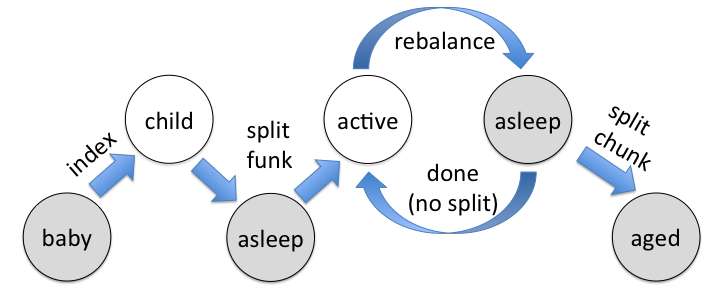
\includegraphics[width=.8\columnwidth]{state-diagram.png}
}
\caption{Chunk life cycle; immutable states are grey and mutable ones are white.
Chunk splits  create new chunks in immutable \emph{baby} state, which changes to the mutable \emph{child} state once they 
are indexed. When the appropriate funks are created, the chunks become \emph{active}. All rebalance operations go through an 
\emph{asleep} state when the chunk is immutable.}
\label{fig:chunklife}
\end{figure}
}

If a munk rebalance exceeds some capacity threshold in a new munk, it triggers a \emph{split}. Unlike 
single-chunk rebalances, splits entail changes in the chunks linked list as well as the index, and so are more subtle. 
A split proceeds in two phases. In the first, the chunk is immutable, namely,  rebalanceLock is held in exclusive mode. In the second (longer) phase, the new chunks are mutable.

The first phase runs in-memory and so is fast (this prevents blocking puts for a long time). 
It proceeds as follows: 
(1) split the munk into two sorted and compacted halves; 
(2) create two new chunks (metadata), each referencing one of the new munks but temporarily sharing the same old funk, both immutable, with the first half munk pointing to the second; 
(3) insert the new chunks into the list instead of the old chunk; and finally  
(4) update the index.
Note that once the new chunks are added to the list they can be discovered by concurrent operations.
On the other hand, other concurrent operations might still access the  old chunk via the index or stale pointers. 
This does not pose a problem because the chunks are immutable and contain the same KV pairs. 

In the second phase, puts are enabled on the new chunks (rebalanceLock is released)
but the new chunks cannot yet be rebalanced. 
Note that the old chunk remains immutable; it continues to serve ongoing reads as long as 
there are outstanding operations that hold references to it, after which it may be  garbage collected.
This phase splits the shared funk. It uses the sorted prefixes of the new munks as SSTables and their 
suffixes as  logs. Once done, the funk references in the new chunks are flipped and future rebalances are allowed.



\remove{
In order to guarantee correctness of this multi-step process, we model a chunk's life cycle as a finite state machine, 
depicted by Figure~\ref{fig:chunklife}. A new chunk is created in \emph{baby} state, in which it is immutable. Once added 
to the index, a chunk transitions to \emph{child} state, in which it is mutable but cannot be rebalanced yet. Finally, when 
a chunk gets its own funk it becomes \emph{active} -- i.e., eligible for all operations. A chunk that has been split into 
two new chunks becomes \emph{aged} -- a state in which it remains immutable but can serve the gets and the scans 
that are concurrently accessing it via the index. Once it gets removed from the chunk list and has no outstanding
reads, it can be disposed. 
%We omit the formal correctness proof for lack of space; see~\cite{kiwi} for similar proofs.   
}

Underflowing neighboring chunks (e.g., following massive deletions) can be merged via a similar protocol. 
Our current \sys\/ prototype does not implement this feature. 
%Merges can be handled the same way by making the two merged munks immutable for the duration of the switch; 
%we do not implement this feature in our prototype.

\subsection{Disk flushes and recovery}
\label{ssec:flush-recovery}

Recall that all puts write to the funk log, regardless of whether the chunk has a munk. 
Funk logs are not replayed on recovery, and so recovery time is not impacted by 
their length.

Like most popular KV-stores, \sys\ supports two modes of persistence -- \emph{synchronous} and \emph{asynchronous}. 
In the former,  updates are persisted to disk (using an \code{fsync} call)
before returning to the user. %, ensuring the written data will survive failures once the operation completes. 
The drawback of this approach is that it is roughly an order-of-magnitude slower than the asynchronous mode.
% in existing KV-stores like RocksDB~\cite{RocksDB} as well as in \sys. 
%In asynchronous mode, updates to funk logs are passed to the OS but might .. 
%are guaranteed to be  persisted only after an explicit \code{fsync} call.  
Asynchronous I/O, where \code{fsync} is only called periodically, 
reduces write latency and increases throughput, but 
may lead to loss of data that was written shortly before a crash. The tradeoffs between the two approaches are 
well known, and the choice is typically left to the user.

\paragraph{Recovery semantics.}
In the synchronous mode, 
%every put operation performs a flush after writing the data in the appropriate funk's \code{log}, and then returns. 
%This ensures that 
the funks always reflect all completed updates. In this case, recovery is straightforward: we simply construct
the chunks linked list and chunk index from the funks on disk, and then the database is immediately ready to serve new requests, populating munks and Bloom filters on-demand.  

In the asynchronous mode, some of the  data written before a crash may be lost, but we  
ensure that the data store consistently reflects a \emph{prefix} of the  values written.
For example, if \DIFdelbegin %DIFDELCMD < \code{put(k1, v1)} %%%
\DIFdel{completes before }%DIFDELCMD < \code{put(k2, v2)} 
%DIFDELCMD < %%%
\DIFdelend \DIFaddbegin \DIFadd{put(k1, v1) completes before put(k2, v2) 
}\DIFaddend is invoked and then the system crashes, then following the recovery, 
if \code{k2} appears in the data store, then \code{k1} must appear in it as well. 
%conversely, if the update of \code{k1}  is lost, \code{k2}  must be also excluded.
Such recovery to a consistent state is important, since later updates may depend on earlier ones. 

Note that the temporal organization in LSMs inherently guarantees such consistency, whereas with spatial data organization,
extra measures need to be taken to ensure it.

\paragraph{Checkpointing for consistent recovery.}

We use \emph{checkpoints} to support recovery to a consistent state in asynchronous mode.
A background process creates checkpoints using atomic scans: 
It first fetches-and-increments GV to obtain a snapshot version \code{gv}.  Next, 
it synchronizes with pending puts via PO to ensure that all puts with smaller versions are complete. 
It then calls \code{fsync} to flush all pending writes to disk.
Finally, it writes \code{gv} to a dedicated \emph{checkpoint file} on disk.
This enforces the following correctness invariant: at all times, all updates pertaining to versions smaller 
than or equal to the version recorded in the checkpoint file have been persisted.
%indicating that all updates pertaining to versions smaller than or equal to this version have been persisted.
Note that some puts with higher versions than \code{gv} might be reflected on disk while others are not. 

\sys's recovery is lazy. 
%All data is initially on disk, and 
Data is fetched into munks as needed during normal operation. 
To ensure consistency, following a recovery,  
retrievals from funks should ignore newer versions that were not included in the latest completed checkpoint before the crash. 
This must be done by every operation that reads data from a funk, namely get or scan from a chunk without a munk, 
funk rebalance, or munk load. 

To facilitate this check, we distinguish between pre-crash versions and new ones created after recovery using \emph{epoch numbers}. 
Specifically, a version is split into an epoch number (in our implementation, the four most-significant bits of the version) and a per-epoch version number. 
Incrementing the GV in the normal mode effectively increases the latter.
The recovery procedure increments the former and resets the latter, so 
versions in the new epoch begin from zero. 

We maintain a \emph{recoveryTable} mapping each recovered epoch to its last checkpointed version number. 
For example, Table~\ref{table:recovery} shows a possible state of the recovery table after two recoveries, i.e., during epoch $2$. 

\begin{table}
\begin{center}
%\small
\begin{tabular}{ll}
epoch & last checkpointed version \\
\hline
0 & 1375\\
1 &  956\\
\end{tabular}
\end{center}
\caption{Example recovery table during epoch $2$.}
\label{table:recovery}
\end{table} 

 \remove{
Every read from a funk  %(during get,  scan, funk rebalance,  or munk load) 
refers to the recovery table in order to identify versions that should be ignored -- 
these are versions from old epochs that exceed the checkpoint number for their epoch. 
}
%\paragraph{Recovery procedure.} 
The recovery procedure reads the checkpoint time from disk, loads the recoveryTable into memory, adds a new row to it with the last epoch and latest checkpoint time, and persists it again. It then increments the epoch number and resumes normal operation with version  $0$ in the new epoch.









\section{Implementation}
\label{sec:impl}
We implement \sys\ in C++. We borrow the \code{SSTable} implementation from the RocksDB open source~\cite{RocksDB}.
Similarly to RocksDB, we use \code{jemalloc} for memory allocation.  

The chunk index is implemented as a sorted array holding the minimal keys of all chunks.  
Whenever a new chunk is created (upon split), the index is rebuilt and the reference to the index is atomically flipped. 
We found this simple implementation to be fastest since splits are infrequent. 

\remove{
\paragraph{Synchronization data structures.}
%We note that 
Using a single pending array to synchronize all
operations can cause unnecessary contention.
We mitigate this problem in our implementation by maintaining two data structures for coordinating different operations
 (similar to~\cite{kiwi}). The first is a per-chunk pending put array (\emph{PPA}) which 
either indicates the current update's key and version, or indicates that the thread is currently not performing a put.
%maps each thread either to a cell in the chunk that the thread is currently attempting to put into and a corresponding version, or an indication that the thread is currently not performing a put. 
The second is a global pending scan array (\emph{PSA}) which tracks versions used by pending scans for compaction purposes; each entry consists of a version \code{ver} and a sequence number \code{seq}, as well as the scan’s key range. Each entry in the \code{PPA}s and \code{PSA} includes, in addition to the operation metadata, an ABA sequence number. 

A put operation consists of 5 phases: (1) \emph{pre-process} - locate the target chunk; if a munk exists, prepare a cell to insert the value into; (2) \emph{publish} - obtain a version while synchronizing with concurrent scans and rebalances via the chunk's lock and publish indication in the chunk's \code{PPA}; (3) \emph{persist} - write the data into the log, indicate it is persisted in the \code{PPA}; (4) \emph{link} - if a munk exists, connect the new cell to the linked list, so it can be found through the list traversal, otherwise, update the row cache to latest version if key is present in the cache; and finally (5) \emph{clean} - clear the entry in the chunk's \code{PPA}, and increase the entry's ABA number.
If the put fails to acquire the chunk's lock (since it is being rebalanced), the operation restarts, and {\inred{re-attempts to}} find an active chunk.
Puts trigger both munk and funk rebalances. The former are handled inline when the munk {\inred{is close to overflow}}; the latter are done in the background 
by helper threads.

%Thus the version number is composed of the GV and 
A per-chunk linearization counter is used to determine the order of concurrent put operations updating the same key.  
Note that multiple \emph{generations} of munks may exist for a chunk throughout its life time.
Therefore, the linearization counter is composed of three parts: (a) the GV value; (b) a \emph{generation number} - incremented whenever a munk is cached into memory and when the munk is rebalanced; and (c) a \emph{sequence number} - incremented upon each put and set to the number of KV-pairs in a munk upon a new generation number. When a new chunk is created as a result of a split, the children chunks inherit their generation number from their parent. The linearization counter is written both to the \code{PPA} upon publishing the put operation, and to the \code{log} when persisting the data. This ensures all operations see the same order of writes per key.

A scan operation first publishes its intent to obtain a version in the \code{PSA}. It determines its scan time $t$ by increasing GV and writing it to its entry in the \code{PSA}. The scan operation then starts traversing the chunks in its range. For each chunk, it first waits for all put operations that are either with smaller version than $t$ or still have not acquired a version to clear their entry in the \code{PPA} or acquire a larger version. After waiting for all concurrent puts to complete, the scan  can read the range from the chunk. If a munk exists, it simply reads the range from the linked list, skipping versions that are not last before $t$. Otherwise, the scan merges the \code{SSTable} and \code{log} data and reads the range from the result, again skipping the penultimate versions. When the scan completes, it clears the entry in the \code{PSA}, and increases the entry's ABA number. Get operations access neither the \code{PSA} nor the \code{PPA}.% data structures.

A munk rebalance iterates through the \code{PSA} to collect the maximum version number among the active scans that cannot be reclaimed yet. If a scan published its intent in the \code{PSA} but published no version number yet, the rebalance waits until either the version is published or the ABA number in the entry is increased. 
\remove{It then acquires the chunk's lock to block additional put operation. If executing a funk rebalance it also acquires the funk rebalance lock for the chunk. After completing the rebalance operation and placing the new content of the chunk in place including the updated metadata, all locks are promoted.
}
}

%\paragraph{Adaptive mechanisms.} \sys\ applies two dynamic mechanisms that adapt to the workload. 
The munk cache applies an LFU eviction policy. %in which the score is a weighted average of the number of accesses per operation type. 
We use exponential decay to maintain the recent access counts, similar to~\cite{tinyLFU}: periodically, all counters are 
sliced by a factor of two. 
The row cache implements a coarse-grained LRU policy using a fixed-size queue of hash tables. 
New entries are inserted into the head table. Once it overflows, a new empty table is added to the head,
and the tail is discarded. Consequently, lookups for recently cached keys are usually served by the head 
table, and unpopular keys are removed from the cache in a bulk once the tail table is dropped.

The row cache  never holds stale values. %, yet need not contain each and every updated key. 
Therefore, a put updates the cache  whenever a previous version of the updated key is already in the cache. 
But if the key is not in the cache, put does not add it, to avoid overpopulating the cache 
in write-dominated workloads. After a get, the up-to-date KV-pair is added to the head table unless it is already there.
If the key's value already exists in another table, it is shared by the two tables, to avoid duplication.

\remove{
\paragraph{Chunk merges support.}
%\inred{move to conclusion and future work?}
Our current implementation does not support chunk merges (to defragment the store after massive data deletion). This could be done as 
part of the rebalance procedure (see~\cite{kiwi}).
In \sys\ this entails merging the funks of two chunks. As in the split operation, the rebalance first acquires the  rebalance locks of the chunks to be merged---to ensure exclusiveness. The content of the chunks is merged and written into a new chunk. Finally, the rebalance acquires the chunks' locks for the short period in which the content that was added to the chunks during the merge is written to the log of the new chunk, and the new chunk swaps the old chunks in the list.
}

\section{Evaluation}
\label{sec:eval}

The experiment setup is described in~\cref{ssec:setup}. 
We present performance results with production data in~\cref{ssec:prod} and with standard synthetic workloads in~\cref{ssec:synthetic}. 

The baseline for our evaluation is RocksDB -- a mature and widely-used industrial KV-store. 
We use the recent RocksDB release 5.17.2, available Oct 24, 2018.  It is worth noting that RocksDB's performance 
is significantly improved  in this release~\cite{CallaghanCompaction}.   
In~\cref{ssec:pebbles} we compare \sys\ against PebblesDB~\cite{PebblesDB}, a research LSM prototype, and TokuDB~\cite{TokuDB} 
-- the only publicly available KV-store whose design is inspired by B$^\epsilon$-trees. Both  perform significantly worse than RocksDB and \sys, 
motivating our focus on RocksDB.


 
\subsection{Setup}
\label{ssec:setup} 

\paragraph{Methodology.} 
Our hardware is a 12-core (24-thread) Intel Xeon 5  with 4TB SSD disk.  
We run each experiment within a Linux container with 16GB RAM. 
Data is stored uncompressed.
We run 5 experiments for each data point and present the median measurement to eliminate outliers. Since experiments are long, the results vary 
little across runs. In all of our experiments, the STD was within $6.1\%$ of the mean, and in most of them below $3\%$. 

We employ a C++ implementation~\cite{Cpp-YCSB} of YCSB~\cite{YCSB}, the  standard  
benchmarking platform for KV-stores. YCSB provides a set of APIs and a synthetic workload suite inspired 
by real-life applications. In order to exercise production workloads, we extend YCSB to replay log files.

In each experiment, a pool of concurrent worker threads running identical
workloads stress-tests the KV-store. We exercise 12 YCSB workers 
and allow the data store to use 4 additional background threads for maintenance.
We also experimented with different numbers of worker threads, finding similar scalability trends in RocksDB and 
\sys; these results are omitted for lack of space.


\paragraph{Configuration.} 
To avoid over-tuning, all experiments use the data stores' default configurations. For RocksDB, we use the configuration exercised by its public 
performance benchmarks~\cite{RocksDBPerf}. 
We also experimented with tuning RocksDB's memory resources based on its performance guide~\cite{RocksDBMemoryTuning}; 
this had mixed results, improving performance by at most 25\% over the default configuration in some workloads but 
deteriorating it by up to 25\% in others. Overall, the default configuration performed best. 
We fixed the PebblesDB code to resolve a data race reported in the project's repository~\cite{pebbles-git-issue}. 

\sys's default configuration 
allocates 8GB to munks and 4GB to the row cache,
so together they consume 12GB out of the 16GB container. 
The row cache consists of three hash tables.  
The Bloom filters for funks are partitioned 16-way.  
We set the \sys\/ maximum chunk size limit to 10MB, the rebalance size trigger to 7MB, 
the funk log size limit to 2MB for munk-less chunks, and to 20MB for chunks with munks. 
The results of the experiments we ran in order to tune these parameters are omitted due to lack of space.

We focus on asynchronous persistence,  i.e., flushes to disk happen in the background; 
(with synchronous I/O, performance is an order-of-magnitude slower, trivializing the results 
in all scenarios that include puts). 

\subsection{Production data}
\label{ssec:prod}

\begin{figure*}[tb]
\centering
\DIFdelbeginFL %DIFDELCMD < \begin{subfigure}{0.29\linewidth}
%DIFDELCMD < %%%
\DIFdelendFL \DIFaddbeginFL \begin{subfigure}{0.32\linewidth}
\DIFaddendFL 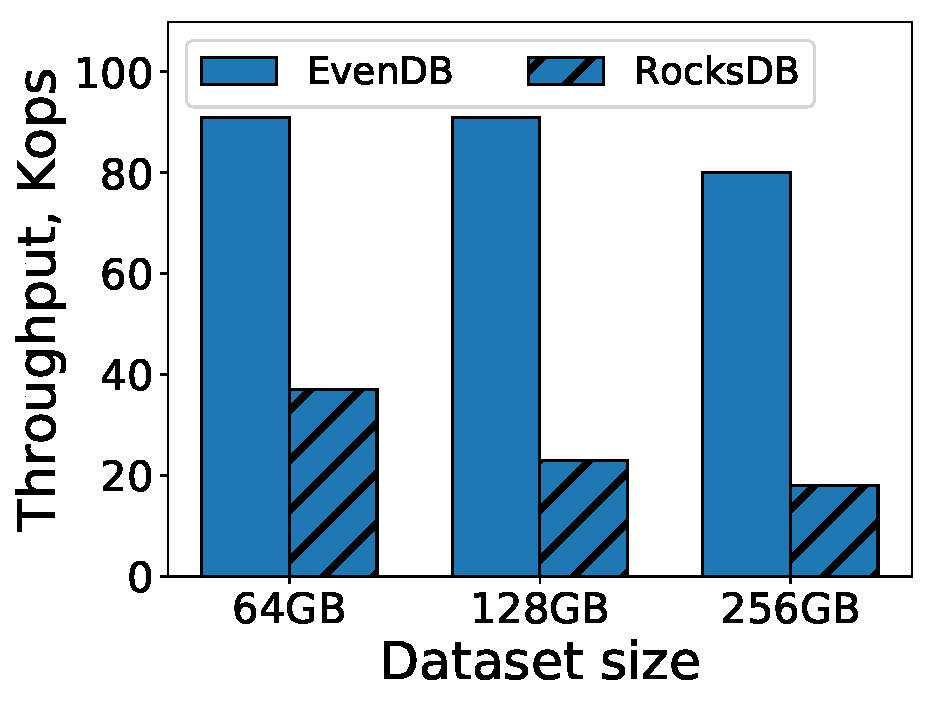
\includegraphics[width=\textwidth]{figs/ingestion.pdf}
\caption{Throughput, Kops}
\label{fig:prod:ingestion:a}
\end{subfigure}
\hspace{0.03\linewidth} 
\DIFdelbeginFL %DIFDELCMD < \begin{subfigure}{0.29\linewidth}
%DIFDELCMD < %%%
\DIFdelendFL \DIFaddbeginFL \begin{subfigure}{0.32\linewidth}
\DIFaddendFL 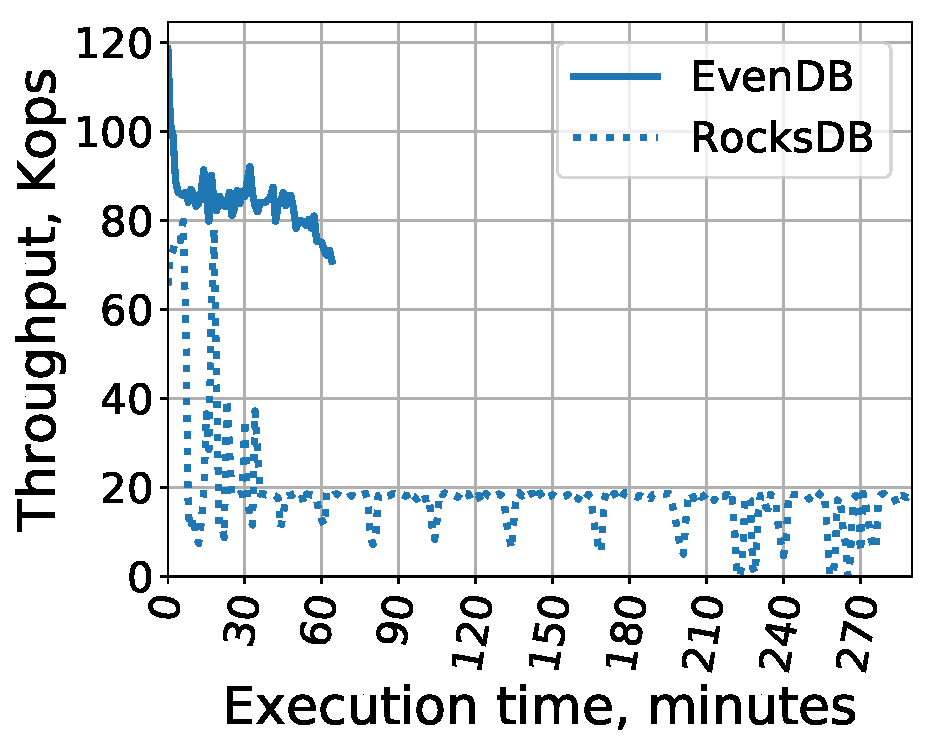
\includegraphics[width=\textwidth]{figs/throughput_256_ingestions_line.pdf}
\caption{Throughput dynamics, 256GB}
\label{fig:prod:ingestion:b}
\end{subfigure}
\DIFdelbeginFL \DIFdelFL{\hspace{0.03\linewidth} 
}%DIFDELCMD < \begin{subfigure}{0.29\linewidth}
%DIFDELCMD < %%%
\DIFdelendFL \DIFaddbeginFL \begin{subfigure}{0.32\linewidth}
\DIFaddendFL 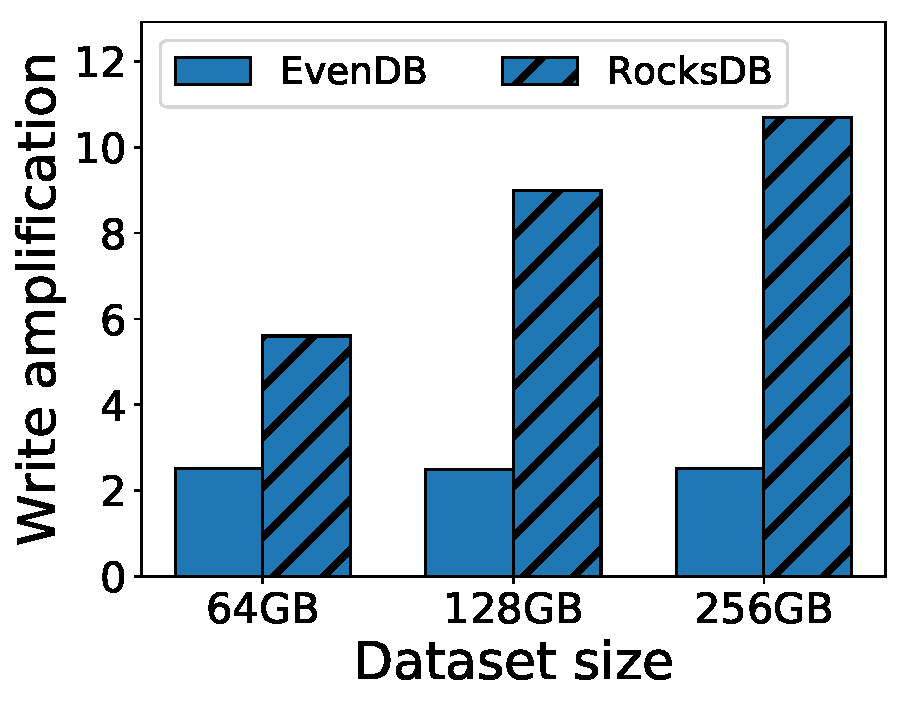
\includegraphics[width=\textwidth]{figs/write_amp_256.pdf}
\caption{Write amplification}
\label{fig:prod:ingestion:c}
\end{subfigure}
\DIFaddbeginFL \DIFaddFL{\hspace{0.03\linewidth} 
}\begin{subfigure}{0.32\linewidth}
	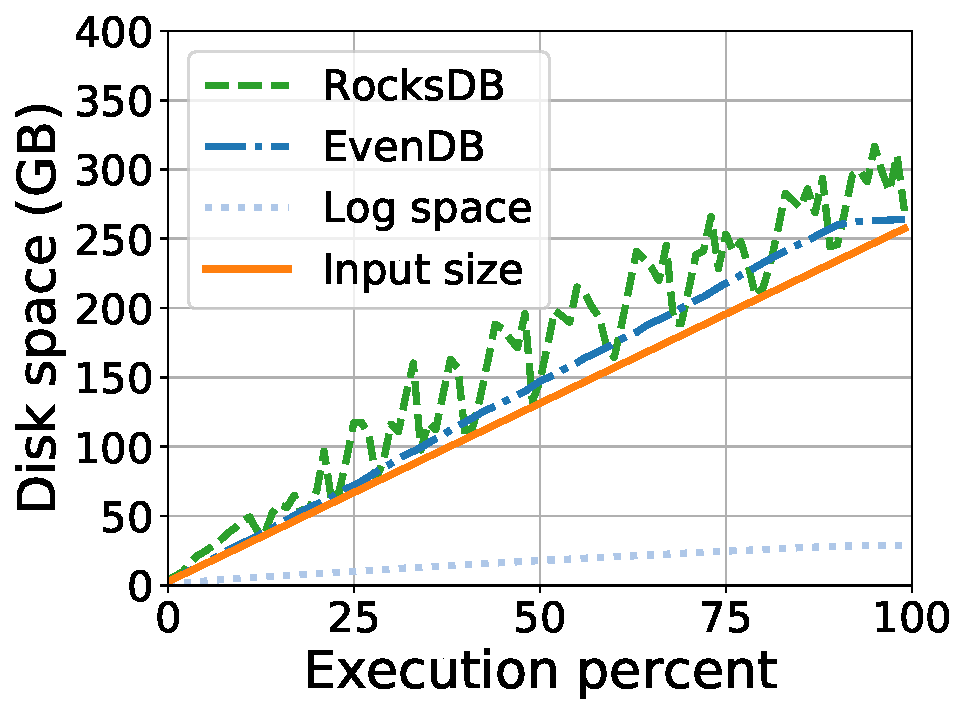
\includegraphics[width=\textwidth]{figs/space_timeline_real_line.pdf}
	\caption{{\DIFaddFL{Space consumption, 256GB}}}
	\label{fig:space_timeline}
\end{subfigure}
\DIFaddendFL \caption{\sys\/ vs RocksDB performance under ingestion (100\% put) workload with production datasets.}
\label{fig:prod:ingestion}
\end{figure*}



\DIFdelbegin %DIFDELCMD < \begin{figure*}[tb]
%DIFDELCMD < \centering
%DIFDELCMD < \begin{subfigure}{0.29\linewidth}
%DIFDELCMD < 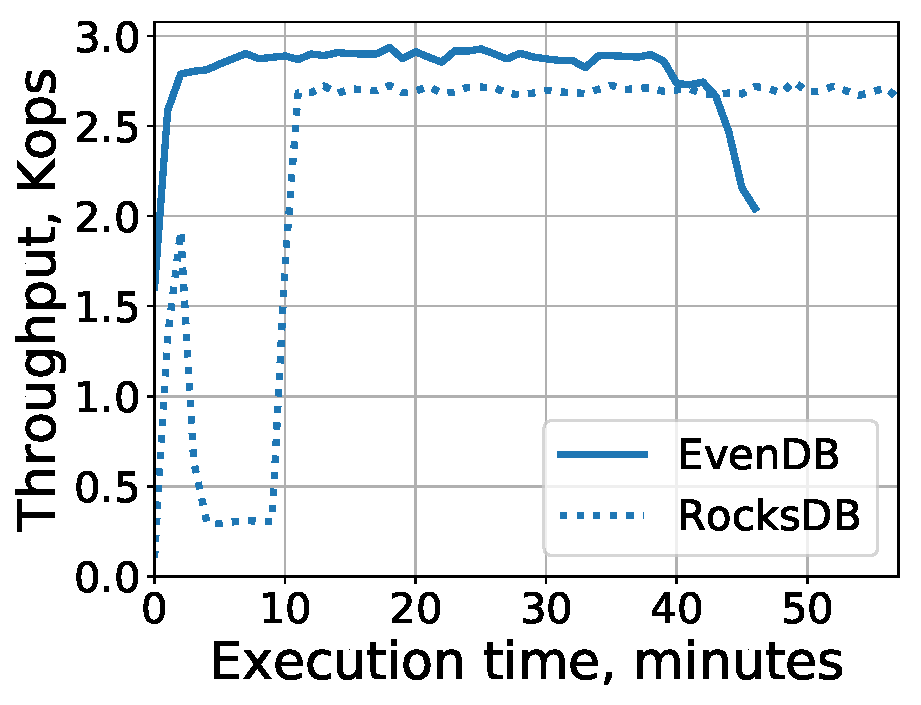
\includegraphics[width=\textwidth]{figs/throughput_64_scans_10s_line.pdf}
%DIFDELCMD < %%%
%DIFDELCMD < \caption{%
{%DIFAUXCMD
\DIFdelFL{64 GB dataset}}
%DIFAUXCMD
%DIFDELCMD < \label{fig:prod:analytics:a}
%DIFDELCMD < \end{subfigure}
%DIFDELCMD < %%%
\DIFdelFL{\hspace{0.03\linewidth} 
}%DIFDELCMD < \begin{subfigure}{0.29\linewidth}
%DIFDELCMD < 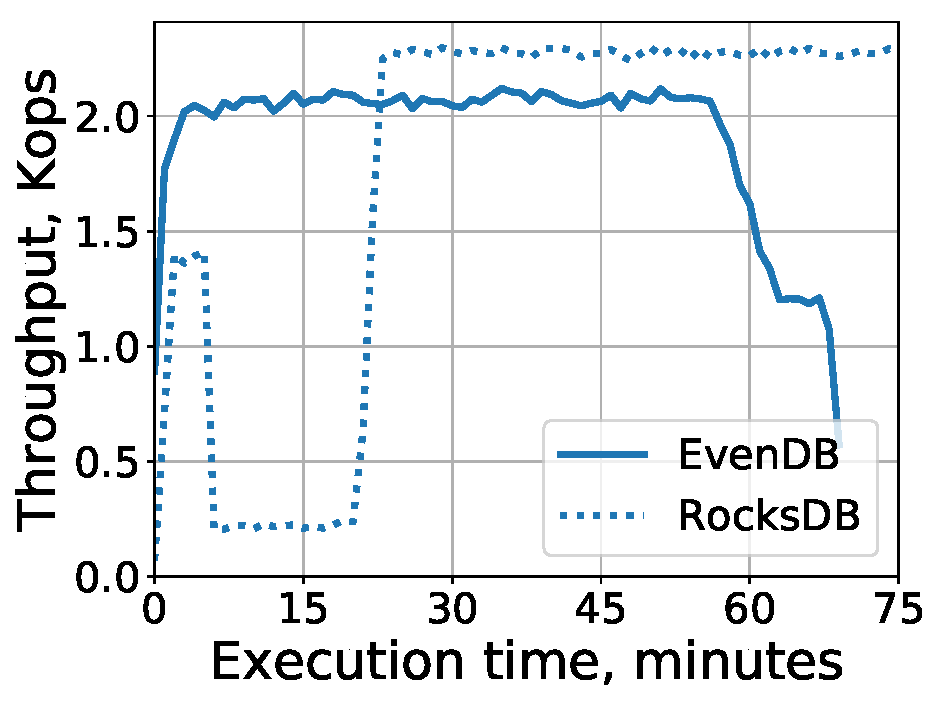
\includegraphics[width=\textwidth]{figs/throughput_128_scans_10s_line.pdf}
%DIFDELCMD < %%%
%DIFDELCMD < \caption{%
{%DIFAUXCMD
\DIFdelFL{128 GB dataset}}
%DIFAUXCMD
%DIFDELCMD < \label{fig:prod:analytics:b}
%DIFDELCMD < \end{subfigure}
%DIFDELCMD < %%%
\DIFdelFL{\hspace{0.03\linewidth} 
}%DIFDELCMD < \begin{subfigure}{0.29\linewidth}
%DIFDELCMD < 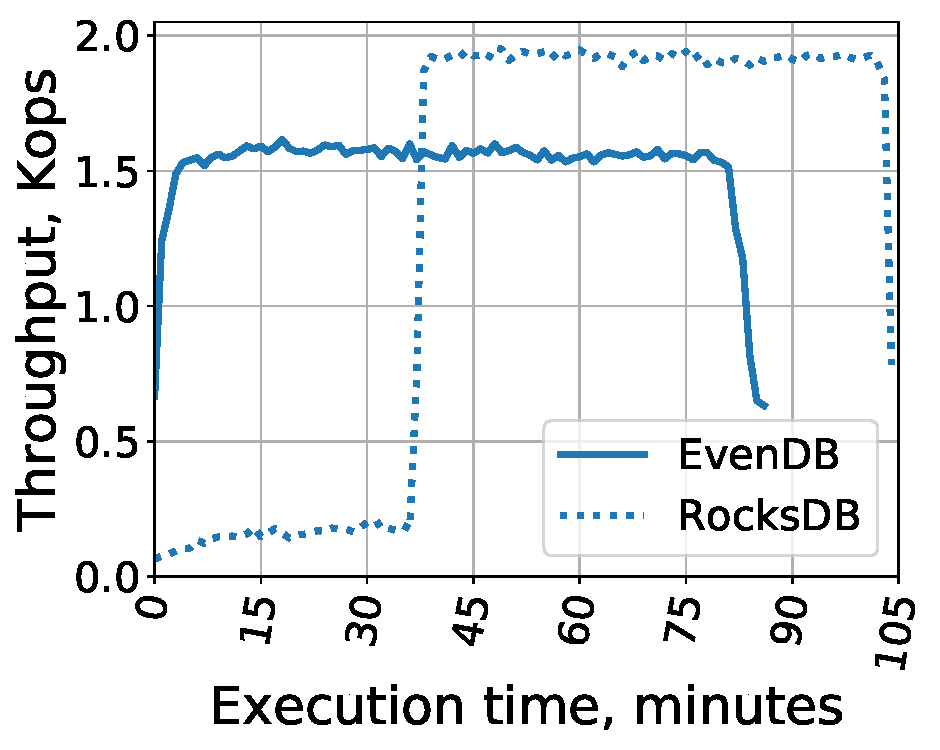
\includegraphics[width=\textwidth]{figs/throughput_256_scans_10s_line.pdf}
%DIFDELCMD < %%%
%DIFDELCMD < \caption{%
{%DIFAUXCMD
\DIFdelFL{256 GB dataset}}
%DIFAUXCMD
%DIFDELCMD < \label{fig:prod:analytics:c}
%DIFDELCMD < \end{subfigure}
%DIFDELCMD < %%%
%DIFDELCMD < \caption{%
{%DIFAUXCMD
\DIFdelFL{\sys\/ vs RocksDB throughput dynamics,  scan-dominated (95\% scans/5\% put) workload with production data.}}
%DIFAUXCMD
%DIFDELCMD < \label{fig:prod:analytics}
%DIFDELCMD < \end{figure*}
%DIFDELCMD < 

%DIFDELCMD < %%%
\DIFdelend Our first set of experiments is driven by a log collected by a production mobile analytics engine. The log captures 
a stream  of $\sim$13M unique events per minute, with an average log record size of 800B, i.e., $\sim$10GB/min. 
We load the logged events into a table indexed by app id and timestamp. 
As noted in~\cref{sec:intro}, the app id distribution is heavy-tailed, i.e., the data exhibits spatial locality. 
We use this log to drive \emph{put-only} (100\% put) and \emph{scan-dominated} 
(95\% scan, 5\% put) tests.

\paragraph{Put-only (data ingestion).} 
\Cref{fig:prod:ingestion} presents our  data ingestion results. 
Here, we load 64GB, 128GB and 256GB of data, in timestamp order; note that this order is different from the KV-store's primary key. 
 \Cref{fig:prod:ingestion:a} depicts the throughput in each experiment. Clearly, \sys\/ is much faster than RocksDB and its advantage 
becomes more pronounced as the dataset grows. For example, \sys\/ ingests 256GB  within 1.1 hours, 
whereas RocksDB requires 4.85 hours (\DIFdelbegin \DIFdel{4.4x }\DIFdelend \DIFaddbegin \DIFadd{$4.4\times$ }\DIFaddend slower). Figure~\ref{fig:prod:ingestion:b} depicts the  
throughput dynamics for the 256GB dataset. RocksDB's throughput, while stable overall, suffers from stalls 
(lasting a minute or longer) caused by compactions. 
%\sys's throughput is noisier, because munk rebalances are more frequent than munk compactions; 
\sys\ delivers predictable performance, with a throughput constantly above \DIFdelbegin \DIFdel{4x }\DIFdelend \DIFaddbegin \DIFadd{$4\times$ }\DIFaddend RocksDB's average rate.

Figure~\ref{fig:prod:ingestion:c} shows the write amplification in the same benchmark. 
While \sys's amplification is unaffected by  scaling, RocksDB deteriorates as the dataset (and consequently, the number of LSM levels) grows. 
%For example, for 256GB RocksDB's amplification factor is 10.7x, whereas \sys's is only 2.5x. 
These results underscore the importance of \sys's in-memory compactions, which consume CPU 
but dramatically reduce the I/O load by minimizing on-disk compaction (funk rebalances). 

This dichotomy between CPU and I/O usage can be observed in 
Table~\ref{fig:io_cpu_bound}, which summarizes  the overall resource consumption in the  256GB ingestion
experiment. We see that \sys\/ is CPU-intensive -- it exploits 40\% more CPU cycles than RocksDB, which means that its average CPU rate is \DIFdelbegin \DIFdel{6.3x }\DIFdelend \DIFaddbegin \DIFadd{$6.3\times$ }\DIFaddend higher. 
On the other hand, RocksDB is I/O-intensive -- it reads \DIFdelbegin \DIFdel{43x }\DIFdelend \DIFaddbegin \DIFadd{$43\times$ }\DIFaddend (!) more data than \sys\/ (recall that the workload is write-only; reading is for compaction purposes). 

\begin{table}[t]
\small
\begin{tabular}{lllll}
%\hline 
& Duration
 &  CPU time  & Read I/O & Write I/O\\
\hline 
\sys &  1.1 hr & 14.6 hr & 	47.6 GB 	&  645.2	GB \\
RocksDB & 4.85 hr & 10.4 hr &  2053.5 GB & 2660.4	GB\\
%\hline 
\end{tabular}
\caption{\sys\/ vs RocksDB resource consumption during ingestion (100\% put) of a 256GB production dataset.}
\label{fig:io_cpu_bound}
\end{table}

\DIFaddbegin \DIFadd{Figure~\ref{fig:space_timeline} shows the disk space used during the ingestion. In \sys\, the space occupied by logs (dotted line) grows linearly with the data size, and is the main reason for space amplification (namely the gap between space consumption and input size). We see the log sizes level out at the end of the run. This occurs because as threads ``run out'' of data to ingest, they can complete a backlog of pending rebalances. 
RocksDB's space consumption increases sharply between compactions and then drops whenever compaction occurs. 
}

\DIFaddend %Indeed, \sys\/ exploits  the workload's spatial locality, and spends most of its time handling RAM-resident data; it hardly 
%ever reads from disk (only upon funk rebalances, which are infrequent). RocksDB, on the other hand, spends a large fraction of its time in 
%compactions, which are insensitive to locality; it re-reads and re-writes the same data many times. 

\begin{figure*}[tb]
\centering
\begin{subfigure}{0.32\linewidth}
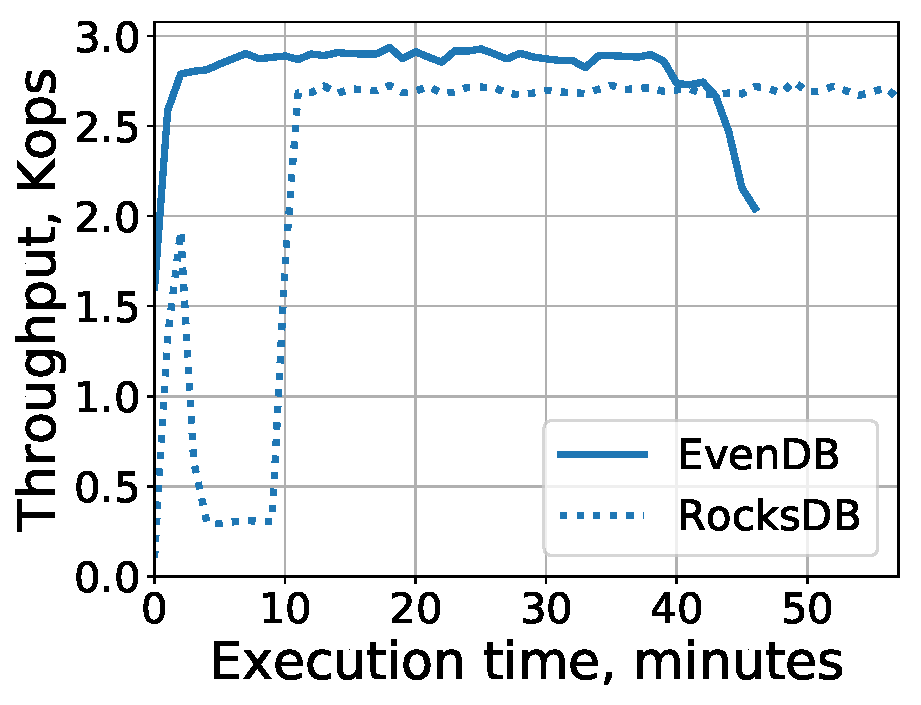
\includegraphics[width=\textwidth]{figs/throughput_64_scans_10s_line.pdf}
\caption{64 GB dataset}
\label{fig:prod:analytics:a}
\end{subfigure}
%\hspace{0.03\linewidth} 
\begin{subfigure}{0.32\linewidth}
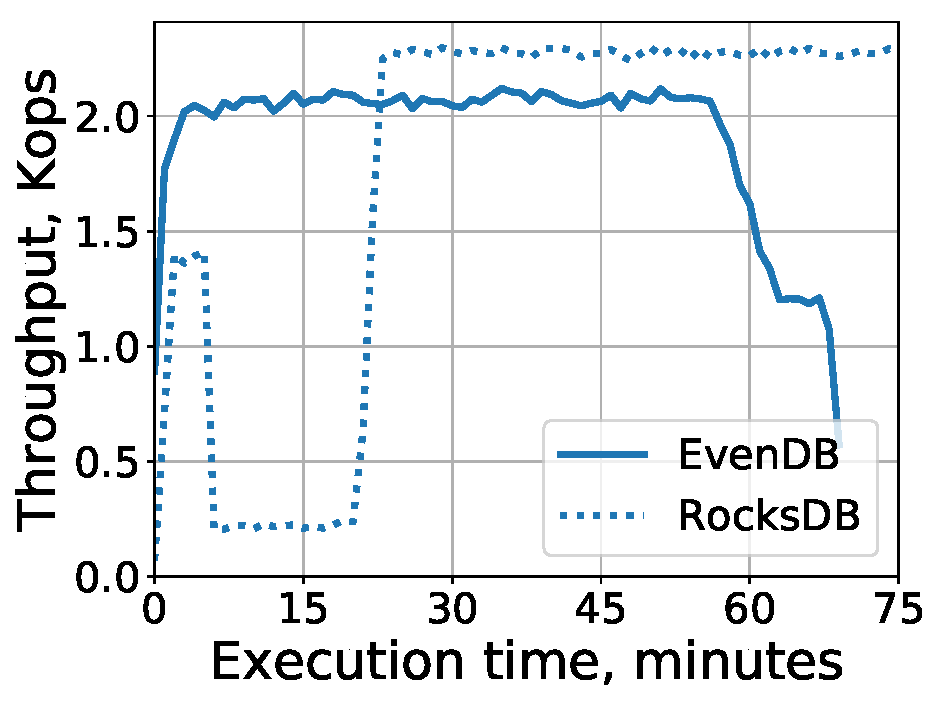
\includegraphics[width=\textwidth]{figs/throughput_128_scans_10s_line.pdf}
\caption{128 GB dataset}
\label{fig:prod:analytics:b}
\end{subfigure}
%\hspace{0.03\linewidth} 
\begin{subfigure}{0.32\linewidth}
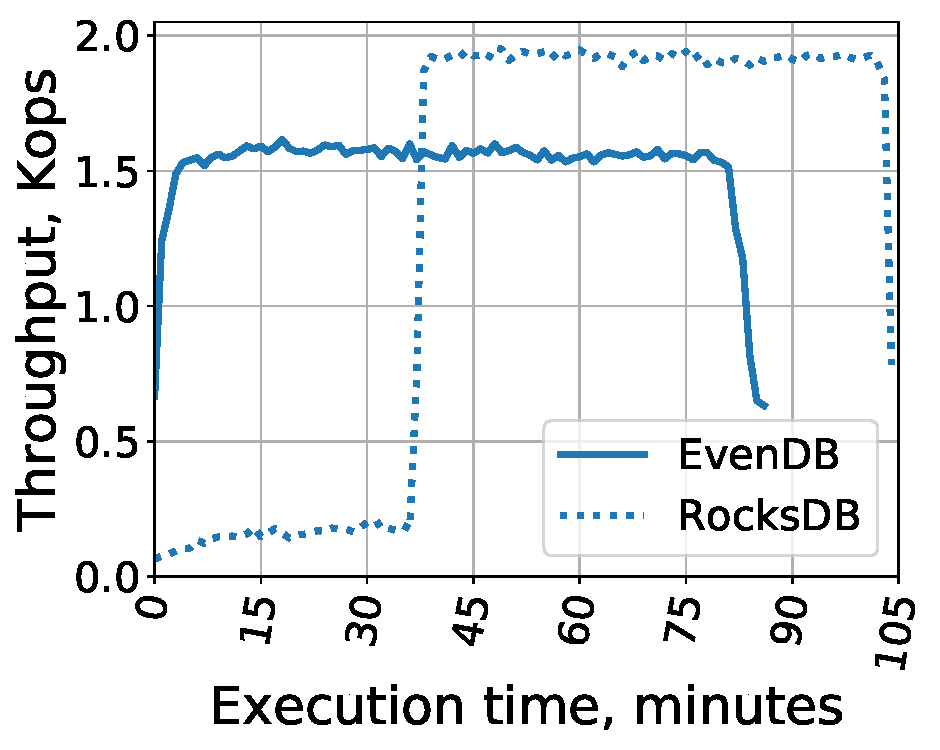
\includegraphics[width=\textwidth]{figs/throughput_256_scans_10s_line.pdf}
\caption{256 GB dataset}
\label{fig:prod:analytics:c}
\end{subfigure}
\caption{\sys\/ vs RocksDB throughput dynamics,  scan-dominated (95\% scans/5\% put) workload with production data.}
\label{fig:prod:analytics}
\end{figure*}

\paragraph{Scan-dominated (analytics).} We run 40M operations -- 95\% range queries, 5\% puts -- 
on the KV-store produced by the ingestion tests.
Every query scans a sequence of recent events within one app (all the scanned rows 
share the  app id key prefix).  
%We study short, medium, and long scans, covering 1 s, 10 s, and 1 min of the app's event history. 
The app id is sampled from the data distribution (so popular apps are queried more frequently).  
Figure~\ref{fig:prod:analytics} depicts the performance dynamics for queries that scan 1-minute histories.
We experimented also with shorter scans, with similar results, which are omitted for lack of space.

\sys\/ completes all experiments 20\% to 30\% faster than RocksDB. 
Yet the two systems' executions are very different. \sys's throughput stabilizes 
almost instantly upon transition from ingestion to analytics because its working set munks are already 
in memory. In contrast, it takes RocksDB 10 to 35 minutes (!) to reach the steady-state performance. 
During this period, it goes through multiple compactions, which degrade its application-level throughput 
beyond 90\%. 

After all compactions are done, RocksDB's improved organization gives it an advantage  over \sys\
(in large datasets) by up to 23\%, because \sys\ searches
in  logs of unpopular funks. We note that this tradeoff between the maintenance cost (for compaction) 
and the scan performance after maintenance  can be controlled via \sys's log size limit parameter.
(E.g., we saw that scan throughput can  grow by up to 20\%  by tuning the system to use 512KB logs instead of
the default 2MB; this experiment is omitted for lack of space.)

%In the long run, %\sys\/ and RocksDB exhibit similar performance under this workload, 
%\inred{RocksDB's performance exceeds \sys's with the large 
%with an eventual advantage to RocksDB in long executions with a large dataset. 
%However, the  dynamics are different.




\subsection{Synthetic benchmarks}
\label{ssec:synthetic} 


In this section, we closely follow the YCSB benchmarking methodology. 
Each experiment first  loads a sequence of KV-pairs, ordered by key, to an initially empty store, then  
runs read operations to warm the caches, and then exercises -- and measures --  the specific experiment 
scenario. Experiments perform 80M data accesses (fewer if some of them are scans). 
Since the load is in key order, the data stores are sorted from the outset, and RocksDB's files cover disjoint key ranges. 
This reduces the overhead of compaction and mitigates the stabilization delay observed in~\cref{ssec:prod}.  Thus, 
performance remains stable throughout the measurement period.

\subsubsection{Workloads}
%\paragraph{Workloads.} 

We vary the dataset size from 4GB to \DIFdelbegin \DIFdel{64GB }\DIFdelend \DIFaddbegin \DIFadd{256GB }\DIFaddend in order to test multiple locality 
scenarios with respect to the available 16GB of RAM. Similarly to the published RocksDB benchmarks~\cite{RocksDBPerf}, 
the keys are 32-bit integers in decimal encoding (10 bytes), which YCSB pads with a 4-byte prefix (so effectively, 
the keys are 14 byte long). Values are 800-byte long. 


% A synthetic workload is defined by  (1)  ratios of get, put, and scan accesses, and (2) a distribution of key access frequencies. 
\noindent
We study the following four key-access distributions:  

%\begin{description}
%\item [Zipf-simple] 
\emph{1. Zipf-simple} -- the standard YCSB Zipfian distribution over simple (non-composite) keys. 
Key access frequencies are sampled from a Zipf distribution\DIFdelbegin \DIFdel{(following~\mbox{%DIFAUXCMD
\cite{Gray:1994:QGB:191839.191886}}\hspace{0pt}%DIFAUXCMD
), with $\theta = 0.8$
(the most popular key 's frequency is  $\sim 0.7\%$).
}\DIFdelend \DIFaddbegin \DIFadd{. 
For most of the experiments, we use the YCSB standard $\ = 0.99$,
(where the most frequent key occurs 4.87\% of the time).
We then study the impact of using a smaller $\theta$, i.e., a less skewed distribution.
%DIF > (following~\cite{Gray:1994:QGB:191839.191886}), with 
}\DIFaddend The ranking is over a random permutation of the key range, so popular keys are uniformly dispersed. % (no spatial locality).
% The key locations are sampled uniformly at random from the whole data range. 
%This workload exhibits medium temporal locality (e.g., the most popular key's frequency is approximately $0.7\%$) and no spatial locality. 
%This is a standard YCSB workload that captures a multitude of use cases  -- e.g., a web page cache distribution by URL. 

%\item [Zipf-composite]  
\emph{2. Zipf-composite} -- a Zipfian distribution over composite keys.
The key's $14$ most significant bits comprise the primary attribute, which  
is drawn from a Zipf (\DIFdelbegin \DIFdel{$\theta=0.8$}\DIFdelend \DIFaddbegin \DIFadd{with the same $\theta$}\DIFaddend ) distribution over its range. The remainder of the key is drawn uniformly at random.
We also experimented with a Zipfian distribution of the key's suffix and 
the trends were similar. %, since performance is most affected by  the primary dimension.
%'s distribution. %Zipf-composite exhibits high spatial locality.% it represents workloads 
%with composite keys.%, such as message threads~\cite{Borthakur:2011:AHG:1989323.1989438},
%social network associations~\cite{Armstrong:2013:LDB:2463676.2465296}, and analytics databases~\cite{flurry},
%and other scenarios with spatial locality of keys, e.g.,  reverse URL domains.

%\item [Latest-simple] 
\emph{3. Latest-simple} -- a standard YCSB workload reading simple keys from a distribution skewed towards recently added ones. 
Specifically, the sampled key's position \DIFdelbegin \DIFdel{wrt }\DIFdelend \DIFaddbegin \DIFadd{w.r.t. }\DIFaddend the most recent key is distributed Zipf. 
%This is with medium spatial and temporal locality, modeling e.g., status updates.

%\item [Uniform] 
\emph{4. Uniform} -- ingestion of keys sampled uniformly at random. RocksDB
reports a similar benchmark~\cite{rocksdb-benchmarks}. %; we present it for completeness.
%\end{description}

The workloads exercise different mixes of puts, gets, and scans. We use standard YCSB scenarios 
(A to F) that range from write-heavy ($50\%$ puts) to read-heavy ($95\%-100\%$ gets or scans). 
%In order to stress the system even more on the write side,
We also introduce a new workload, P, comprised of $100\%$ puts (a data ingestion scenario
as in~\cref{ssec:prod}).
%non-sequential data load scenario (e.g., an ETL from an external data pipeline~\cite{flurry}). 

\subsubsection{Evaluation results}

\begin{figure*}[tb]
\centering
\begin{subfigure}{0.32\linewidth}
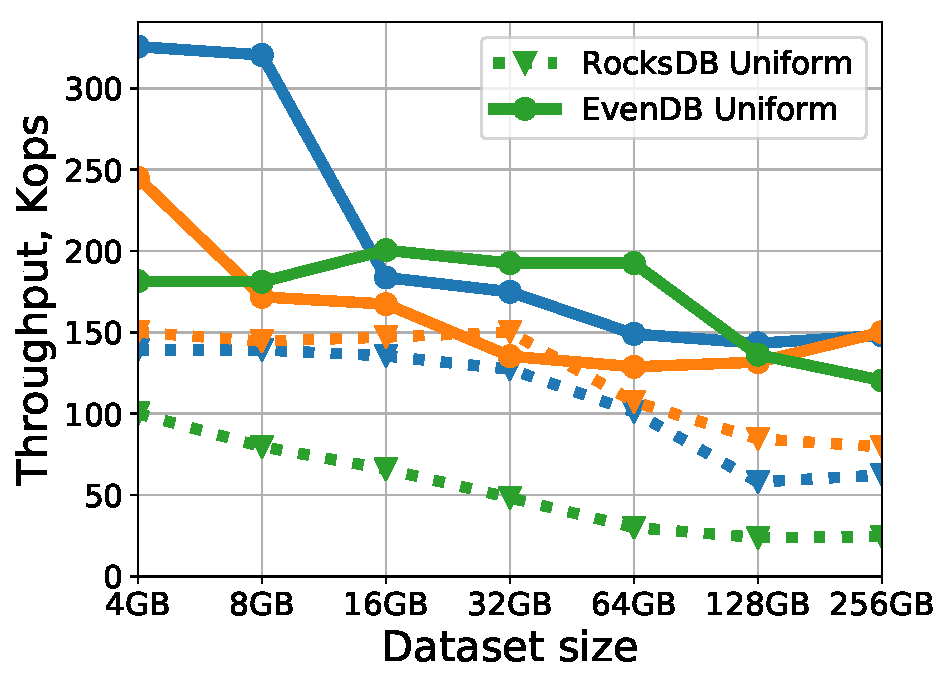
\includegraphics[width=\textwidth]{figs/Workload_P_line.pdf}
\caption{P -- 100\% put}
\label{fig:throughput:p}
\end{subfigure}
%\hspace{0.01\linewidth} 
\begin{subfigure}{0.32\linewidth}
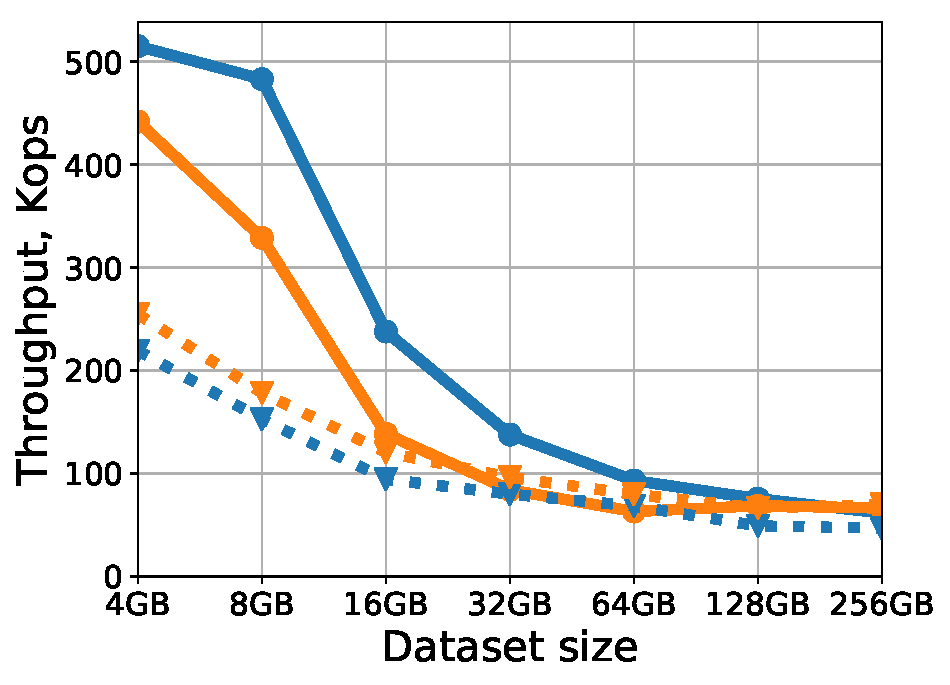
\includegraphics[width=\textwidth]{figs/Workload_A_line.pdf}
\caption{A -- 50\% put, 50\% get}
\label{fig:throughput:a}
\end{subfigure}
%\hspace{0.01\linewidth} 
\begin{subfigure}{0.32\linewidth}
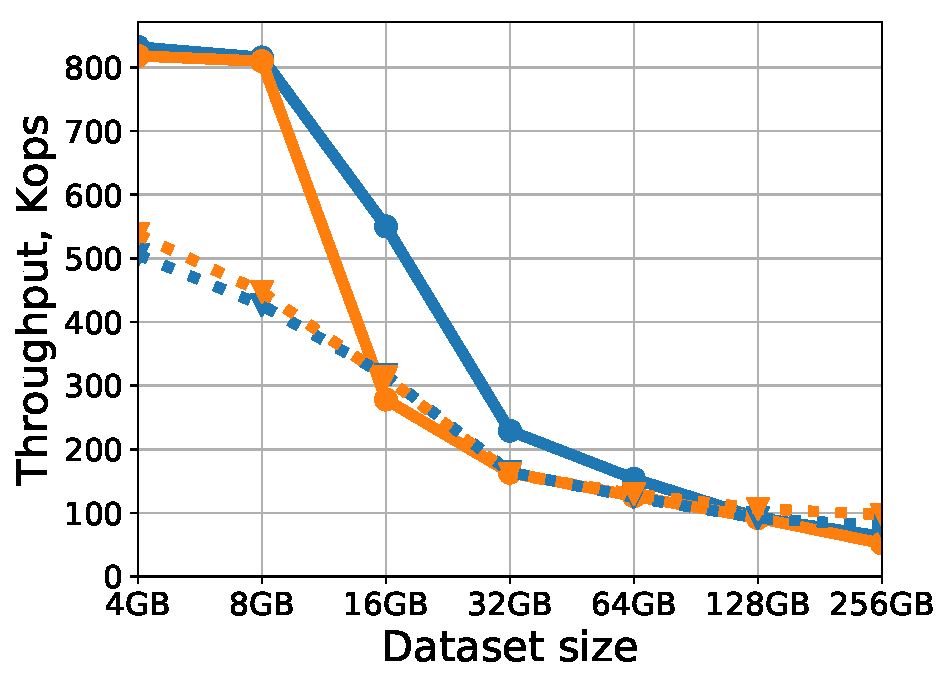
\includegraphics[width=\textwidth]{figs/Workload_B_line.pdf}
\caption{B -- 5\% put, 95\% get}
\label{fig:throughput:b}
\end{subfigure}
%\hspace{70pt}
\begin{subfigure}{0.32\linewidth}
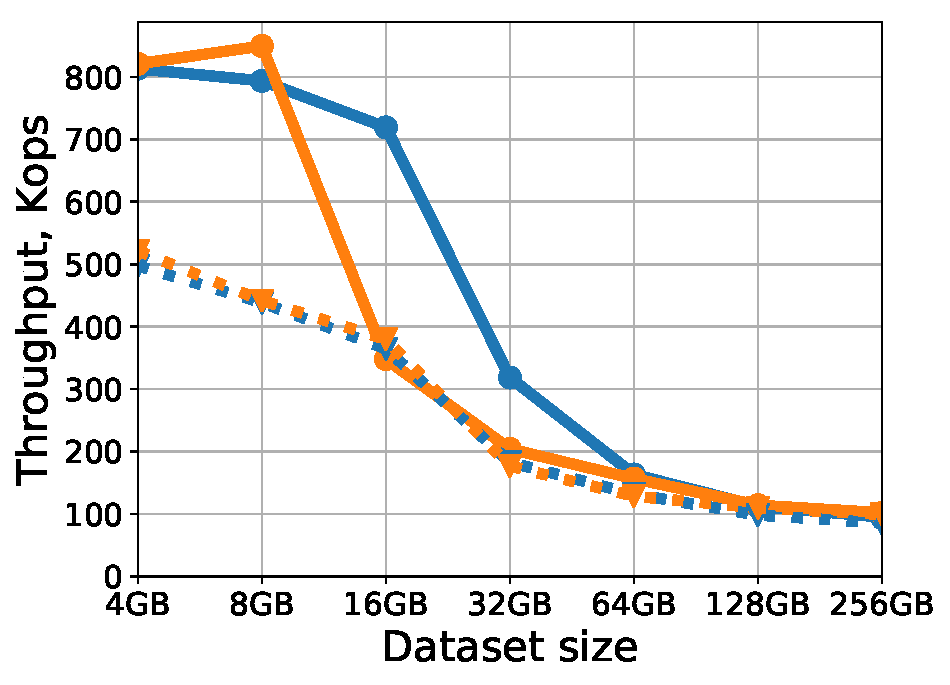
\includegraphics[width=\textwidth]{figs/Workload_C_line.pdf}
\caption{C -- 100\% get}
\label{fig:throughput:c}
\end{subfigure}
\begin{subfigure}{0.32\linewidth}
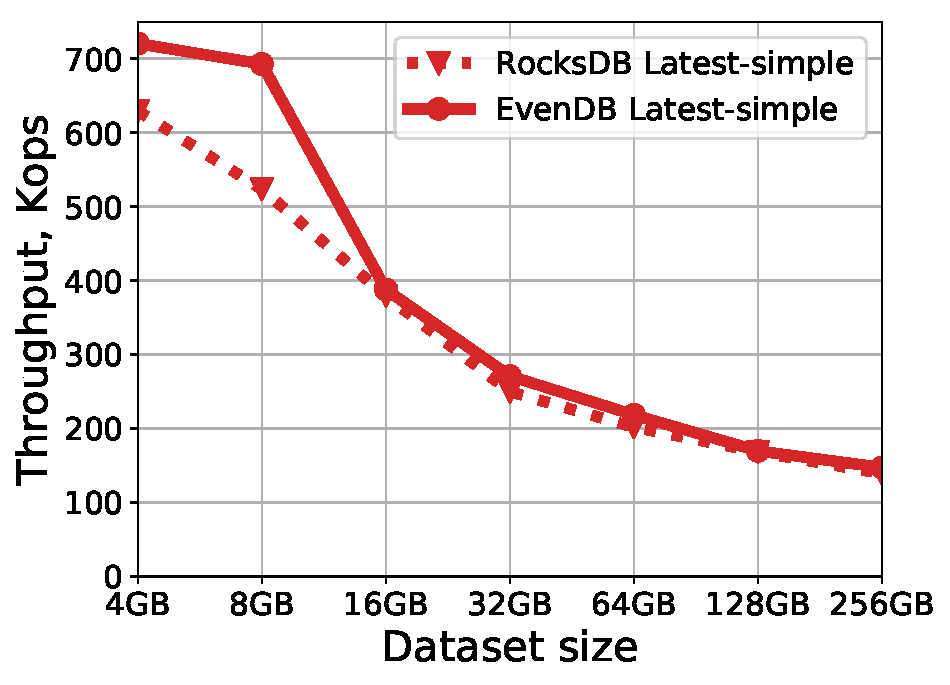
\includegraphics[width=\textwidth]{figs/Workload_D_line.pdf}
\caption{D -- Latest-simple, 5\% put, 95\% get}
\label{fig:throughput:d}
\end{subfigure}
\begin{subfigure}{0.32\linewidth}
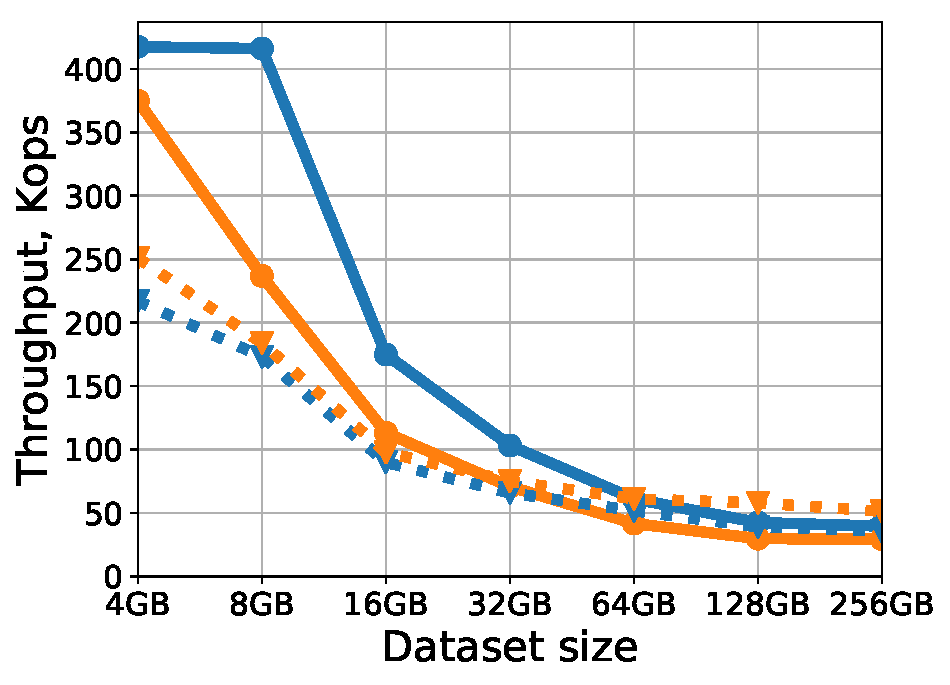
\includegraphics[width=\textwidth]{figs/Workload_F_line.pdf}
\caption{F -- 100\% get-modify-put}
\label{fig:throughput:f}
\end{subfigure}
%\hspace{70pt}
\begin{subfigure}{0.32\linewidth}
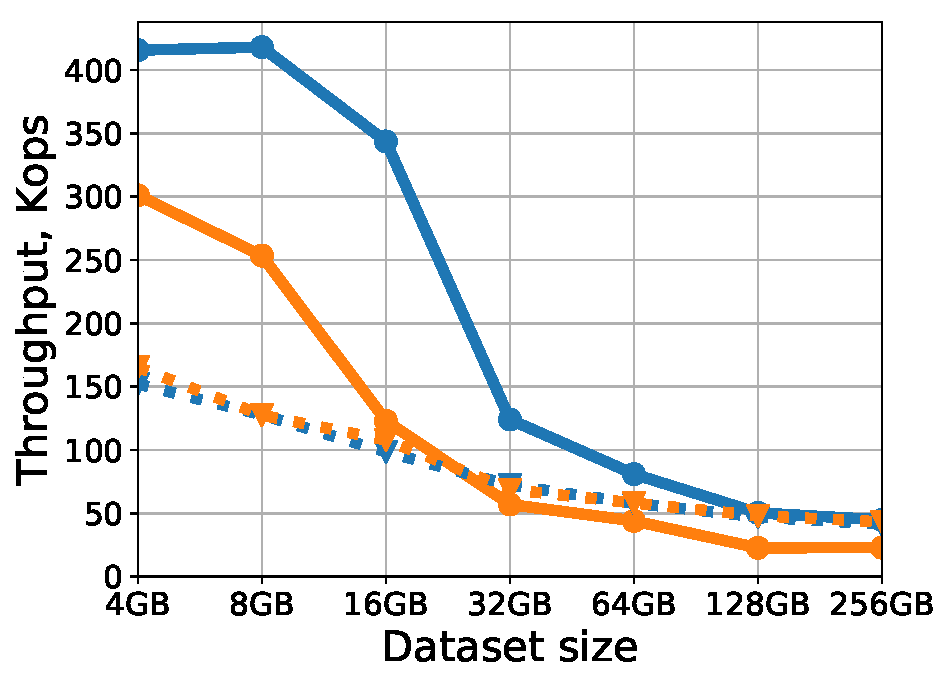
\includegraphics[width=\textwidth]{figs/Workload_E-_line.pdf}
\caption{E10 \\ 5\% put, 95\% scan (10 rows)}
\label{fig:throughput:e10}
\end{subfigure}
\begin{subfigure}{0.32\linewidth}
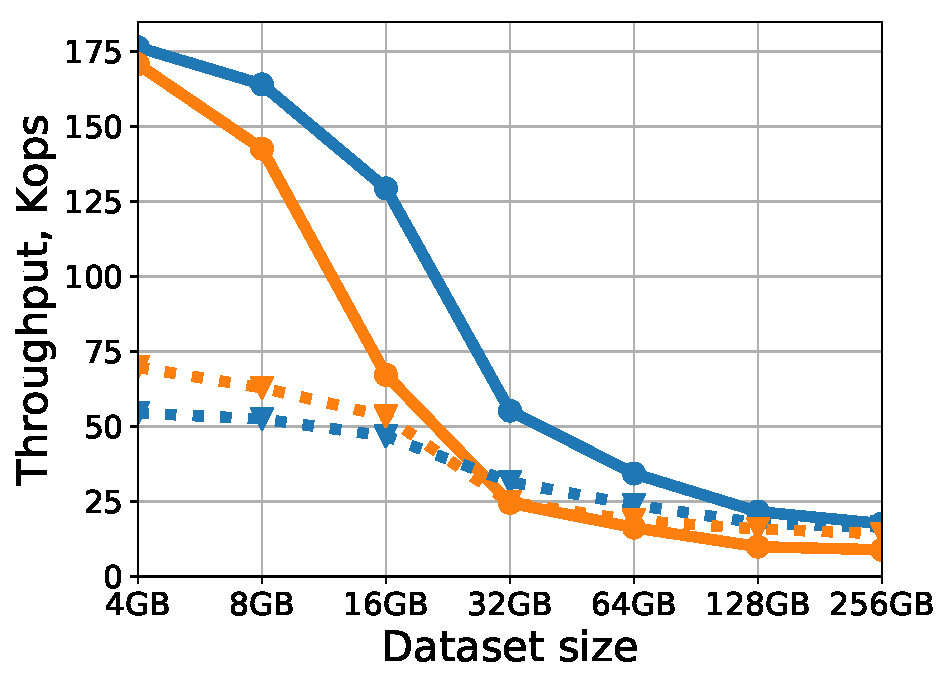
\includegraphics[width=\textwidth]{figs/Workload_E_line.pdf}
\caption{E100 \\ 5\% put, 95\% scan (100 rows)}
\label{fig:throughput:e100}
\end{subfigure}
\begin{subfigure}{0.32\linewidth}
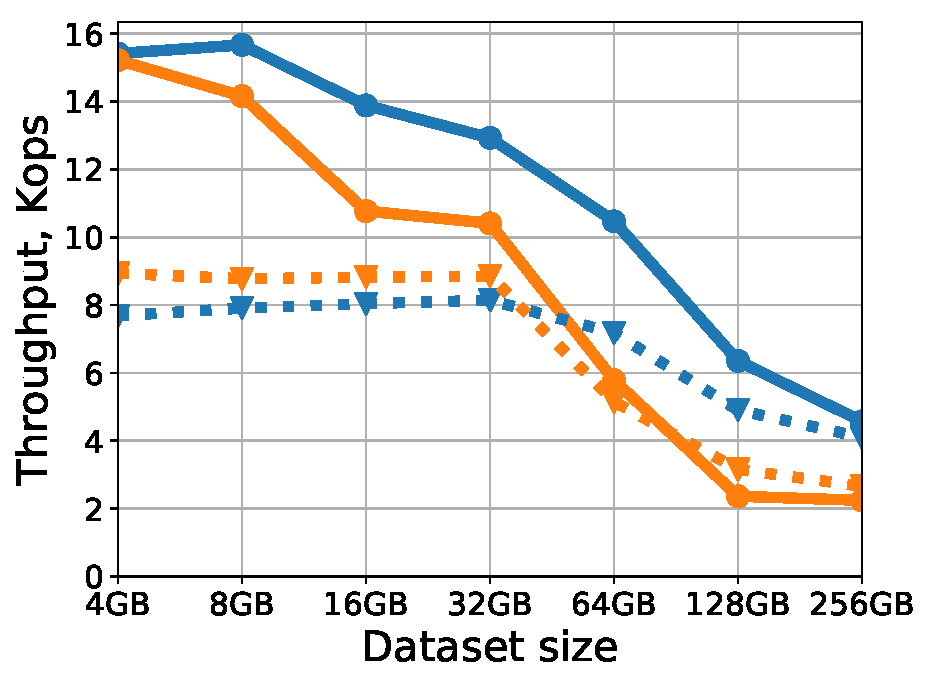
\includegraphics[width=\textwidth]{figs/Workload_E+_line.pdf}
\caption{E1000 \\5\% put, 95\% scan (1000 rows)}
\label{fig:throughput:e1000}
\end{subfigure}
\begin{subfigure}{\linewidth}
\centerline{

\includegraphics[width=0.9\textwidth]{figs/legend.pdf}
\vspace{-5mm}
}
\end{subfigure}
\caption{
{\sys\/ vs RocksDB throughput under YCSB workloads with various key distributions.}
}
\label{fig:throughput}
\end{figure*}

Figure~\ref{fig:throughput} presents the throughput measurements in all YCSB workloads. 
Except for workload D, which exercises the Latest-simple pattern
(depicted in red), all benchmarks are run with both  Zipf-simple (orange) 
and Zipf-composite (blue). The P (put-only) workload 
additionally exercises the Uniform access pattern (green). \sys\/ results are depicted with solid
lines, and RocksDB with dotted lines. 

We now discuss the results for the different scenarios.

\paragraph{Put-only (data ingestion)\DIFaddbegin \DIFadd{.}\DIFaddend } \DIFdelbegin \DIFdel{is tested in }\DIFdelend \DIFaddbegin \DIFadd{In }\DIFaddend workload {P} (100\% put, Figure~\ref{fig:throughput:p})\DIFdelbegin \DIFdel{. 
}\DIFdelend \DIFaddbegin \DIFadd{, 
}\DIFaddend \sys's throughput is \DIFdelbegin \DIFdel{1.8x to 6.4x }\DIFdelend \DIFaddbegin \DIFadd{$1.8\times$ to $6.4\times$ }\DIFaddend that of RocksDB's with uniform keys, \DIFdelbegin \DIFdel{1.3x to 2.3x }\DIFdelend \DIFaddbegin \DIFadd{$1.3\times$ to $2.3\times$ }\DIFaddend with Zipf-composite keys, 
and \DIFdelbegin \DIFdel{0.9x to 1.6x }\DIFdelend \DIFaddbegin \DIFadd{$0.9\times$ to $1.6\times$ }\DIFaddend with Zipf-simple keys. This scenario's bottleneck is the reorganization of persistent data  
(funk rebalances in \sys, compactions in RocksDB), which causes write amplification and hampers performance. 

 Under the Zipf-composite workload, \sys\ benefits from spatial locality whereas RocksDB's write performance 
 is relatively insensitive to it, as is typical for LSM stores. For small datasets (4-8GB), \sys\/ accommodates 
all puts in munks, and so funk rebalances are rare. In big datasets, funk rebalances do occur, but mostly in 
munk-less chunks, which are accessed infrequently. This is thanks to \sys\/'s high log size limit for chunks 
with munks. Hence, in both cases, funk rebalances incur less I/O than RocksDB's compactions, 
which do not distinguish between hot and cold data. 

% Under the Zipf-simple workload, the gains are moderate due to the low spatial locality. They are most pronounced 
% for small datasets that fit into RAM.

The Uniform workload exhibits no locality of any kind. 
 \sys\/ benefits from this because keys are dispersed evenly across chunks, hence all funk logs grow 
 slowly, and funk rebalances are infrequent. The throughput is therefore insensitive to the dataset 
 size. In contrast, RocksDB performs compactions frequently albeit they are not effective (since there are few redundancies). Its throughput 
 degrades  with the data size since when compactions cover more keys they engage more files.


   
The write amplification in this experiment is summarized in 
Figure~\ref{fig:writeamp}. We see that \sys\/ reduces the disk write rate dramatically, 
with the largest gain observed for big datasets (e.g.,  for the 64GB dataset 
the amplification factors are $1.3$ vs $3.1$ under Zipf-composite, and $1.1$ vs $7.6$ under Uniform). 

\DIFaddbegin \DIFadd{We further measured space amplification at the end of the run, and found that both \sys\ and RocksDB have roughly $17\%$ 
space amplification. Note that in \sys, the space amplification is controlled by the log size threshold parameter.
}


\DIFaddend \begin{figure}[t]
	\centering
	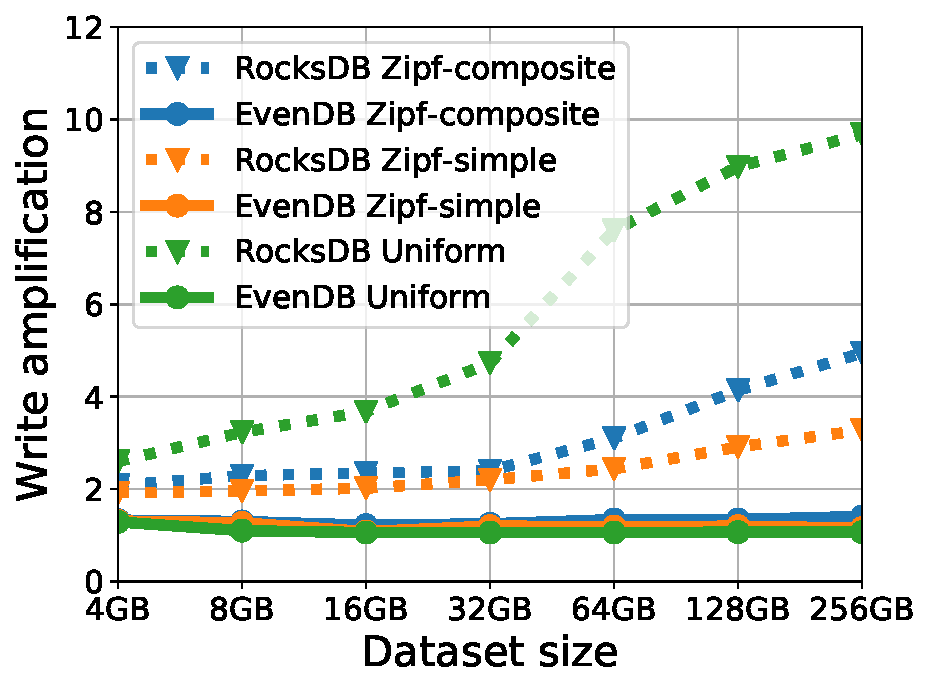
\includegraphics[width=0.4\textwidth]{figs/write_amp_p_line.pdf}
	\caption{{\sys\/ vs RocksDB write amplification under the put-only workload P.}}
	\label{fig:writeamp}
\end{figure}

\paragraph{Mixed put-get\DIFaddbegin \DIFadd{.}\DIFaddend } \DIFdelbegin \DIFdel{is represented in workloads }\DIFdelend \DIFaddbegin \DIFadd{Workloads }\DIFaddend A (50\% put, 50\% get, Figure~\ref{fig:throughput:a}) and 
F (100\% get-modify-put, Figure~\ref{fig:throughput:f}) \DIFaddbegin \DIFadd{invoke puts and gets at the same rate}\DIFaddend . Note that the latter exercises the usual get and put API (i.e., does not provide atomicity). 
\DIFdelbegin \DIFdel{In this scenario, \sys\ works well with composite keys, e.g., in workload A it  achieves $1.4$x to $3.5$x the throughput of RocksDB due to better exploitation of spatial locality. 
With simple keys, on the other hand, the }\DIFdelend \DIFaddbegin \DIFadd{The }\DIFaddend get-put mix is particularly challenging for \sys, \DIFdelbegin \DIFdel{which }\DIFdelend \DIFaddbegin \DIFadd{especially with simple keys, where it }\DIFaddend serves many gets from disk due to the
low spatial locality. The bottleneck is the linear search in funk logs, which  fill up due to the high put rate.
RocksDB's caching is more effective in this scenario, so its disk-access rate in get operations is lower,  resulting in faster gets. 
\DIFdelbegin \DIFdel{Note that \sys\/ is still reasonably close to RocksDB in the worst case 
(0.75x and 0.7x throughput for the 64GB dataset in 
A and F, respectively).
%DIF < (In-memory searches are three orders of magnitude faster.)
}\DIFdelend \DIFaddbegin \DIFadd{While \sys\ continues to outperform RocksDB in small data sets or when spatial locality is high, its performance deteriorates in 
large data sets with no such locality, where RocksDB is almost $2\times$ faster.
}\DIFaddend 

Figure~\ref{fig:tail_latency}, which depicts tail (95\%) put and get latencies in this scenario, 
corroborates our analysis. \sys\/ has faster puts and faster or similar get tail latencies with composite keys
(Figure~\ref{fig:tail_latency:co}). With simple keys (Figure~\ref{fig:tail_latency:si}),  
the tail put latencies are similar in the two data stores, but the tail get latency of \sys\ 
in large datasets surges.

To understand this spike, we break down the get latency in  Figure~\ref{fig:readstat}. 
Figure~\ref{fig:readstat:dist} classifies gets by the storage  component 
that fulfills the request, and Figure~\ref{fig:readstat:lat} presents the disk search latencies by component. 
We see that with large datasets, disk access dominates the latency.
For example, in the 64GB dataset, $3.3\%$ of gets are served from logs under Zipf-composite vs $4\%$ under Zipf-simple,
and the respective log search latencies are $2.6$ ms vs $4.2$ ms. This is presumably because in the latter, puts are more dispersed, 
hence the funks are cached less effectively by the OS, and the disk becomes a bottleneck due to the higher I/O rate.



\begin{figure}[htb]
\centering
\begin{subfigure}{0.49\linewidth}
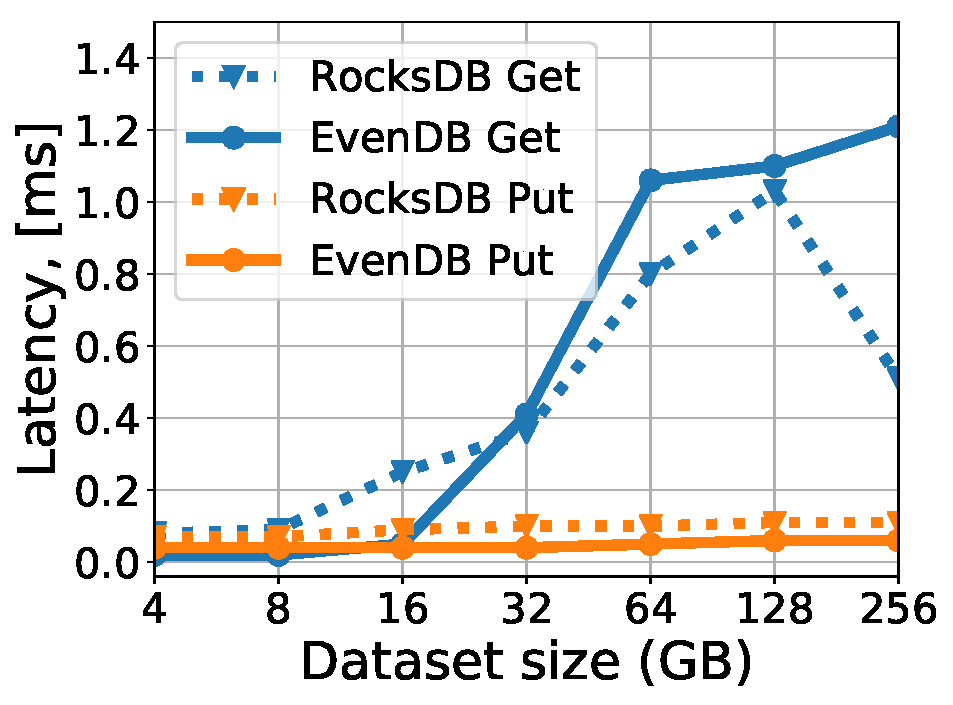
\includegraphics[width=\textwidth]{figs/tail_flurry_line.pdf}
\caption{Zipf-composite}
\label{fig:tail_latency:co}
\end{subfigure}
\begin{subfigure}{0.49\linewidth}
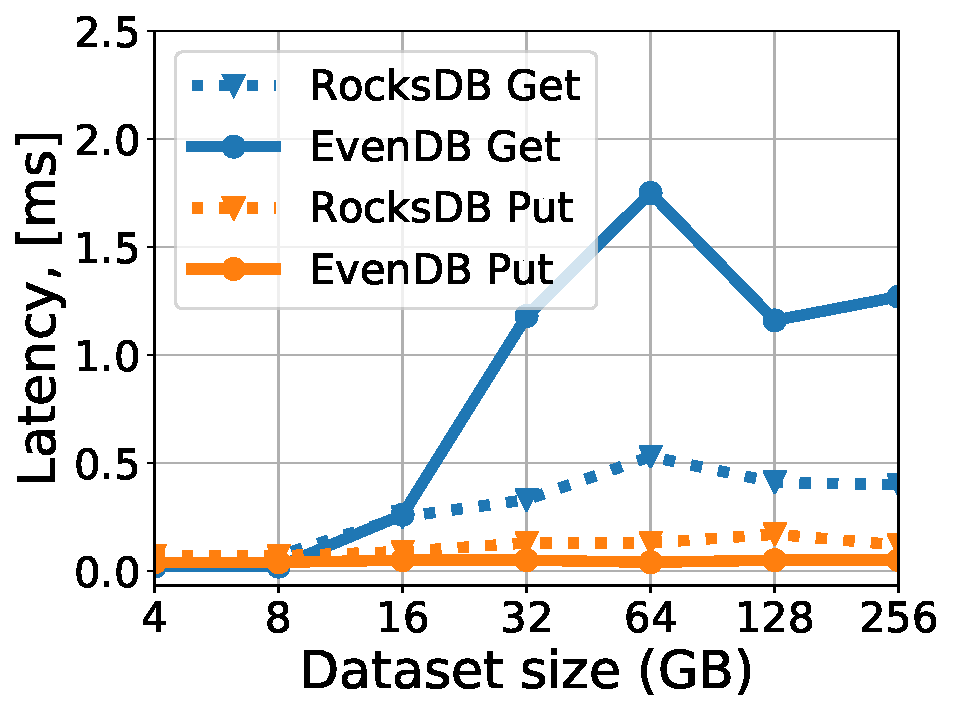
\includegraphics[width=\textwidth]{figs/tail_zipf_line.pdf}
\caption{Zipf-simple}
\label{fig:tail_latency:si}
\end{subfigure}
\caption{{\sys\/ vs RocksDB 95\% latency (ms), under a mixed get-put workload A.}}
\label{fig:tail_latency}
\end{figure}

\begin{figure}[htb]
\centering
%\hspace{0.05\linewidth}
\begin{subfigure}{0.6\linewidth}
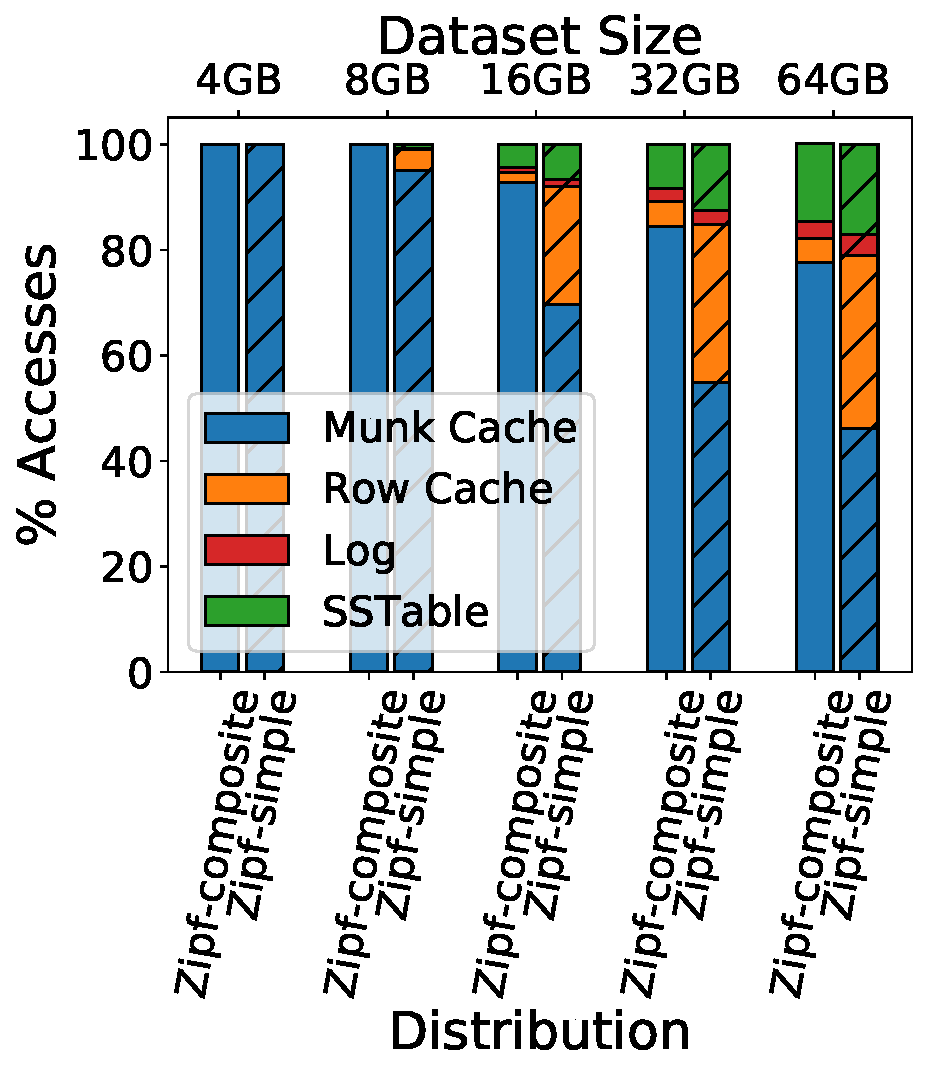
\includegraphics[width=\textwidth]{figs/Time_percentage_A.pdf}
\vskip .1in
\caption{Fraction of get accesses}
\label{fig:readstat:dist}
\end{subfigure}

%\hspace{0.05\linewidth}
\begin{subfigure}{0.6\linewidth}
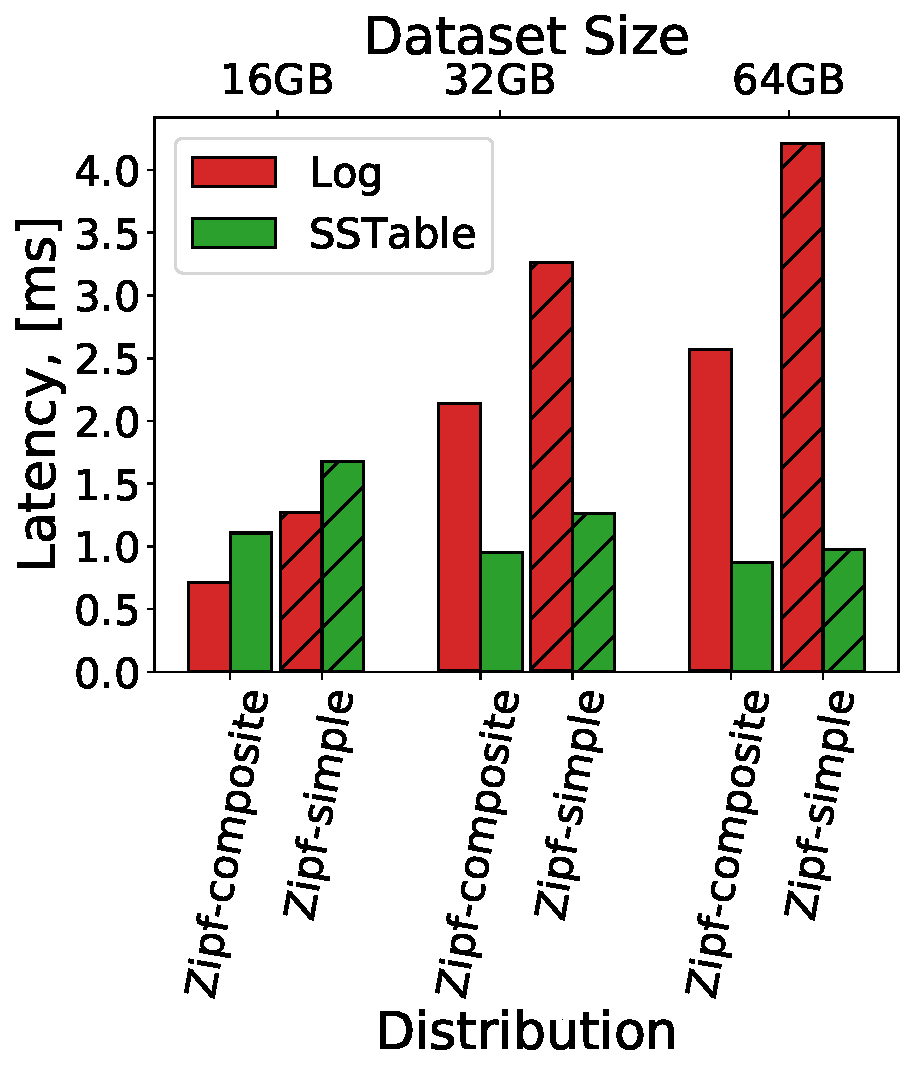
\includegraphics[width=\textwidth]{figs/Latency_A.pdf}
\caption{On-disk get access latency}
\label{fig:readstat:lat}
\end{subfigure}
\caption{{\sys\/ get latency breakdown by serving component, under a mixed get-put workload A.}}
\label{fig:readstat}
\end{figure}

The figure also shows that the row cache becomes instrumental as spatial locality drops -- it serves $32.8\%$ of gets with Zipf-simple 
vs $4.5\%$ with Zipf-composite. 

\DIFdelbegin \paragraph{\DIFdel{Get-dominated}} 
%DIFAUXCMD
\addtocounter{paragraph}{-1}%DIFAUXCMD
\DIFdel{workloads (B--D, }\DIFdelend \DIFaddbegin \DIFadd{Workloads B and D (}\DIFaddend Figures~\ref{fig:throughput:b} \DIFdelbegin \DIFdel{--\ref{fig:throughput:d}) are 
favorable to 
\sys, which }\DIFdelend \DIFaddbegin \DIFadd{and~\ref{fig:throughput:d}) also mix gets and puts, but with a lower put rate. 
Here, the funk logs don't grow as quickly as under an even put-get mix, and 
\sys\  }\DIFaddend has a marked advantage in all key distributions with small datasets (up to the available RAM size) 
and also with Zipf-composite \DIFaddbegin \DIFadd{and Latest-simple }\DIFaddend keys in large datasets. \DIFdelbegin \DIFdel{For example, in }\DIFdelend \DIFaddbegin \DIFadd{But here, too, its advantage diminishes with the data set size,
especially under the Zipf-simple key distribution.  
}

\paragraph{\DIFadd{Read-only.}} 
\DIFadd{In }\DIFaddend workload C (100\% get, Figure~\ref{fig:throughput:c}), 
\sys\/ performs \DIFdelbegin \DIFdel{$1.2$x to $2$x }\DIFdelend \DIFaddbegin \DIFadd{$1.1\times$ to $2\times$ }\DIFaddend better than RocksDB with composite keys, and up to \DIFdelbegin \DIFdel{$1.9$x  }\DIFdelend \DIFaddbegin \DIFadd{$1.9\times$  }\DIFaddend with simple ones (for small datasets). 
In these scenarios, \sys\  manages to satisfy most gets from munks, resulting in good performance.
RocksDB relies mostly on the OS cache to serve these requests and so it pays the overhead for invoking system calls. 
%DIF < As we discuss in~\S\ref{ssec:drill} below, 
RocksDB's performance in this scenario can be improved by using a larger application-level block cache,
but \DIFdelbegin \DIFdel{this }\DIFdelend \DIFaddbegin \DIFadd{our experiments (not presented in this paper) have shown that this }\DIFaddend hurts performance for bigger datasets as well as in other benchmarks.
\DIFdelbegin \DIFdel{(These results are not elaborated due to space limitations). 
}\DIFdelend 


\paragraph{Scan-dominated\DIFaddbegin \DIFadd{.}\DIFaddend } \DIFdelbegin \DIFdel{benchmarks (}\DIFdelend \DIFaddbegin \DIFadd{Benchmarks }\DIFaddend E10--1000  \DIFdelbegin \DIFdel{,  }\DIFdelend \DIFaddbegin \DIFadd{(}\DIFaddend 5\% put, 95\% scan, Figures~\ref{fig:throughput:e10}-~\ref{fig:throughput:e1000})
iterate through a number of items sampled uniformly in the range [1,S], where S is  10, 100, or 1000. 
\DIFdelbegin \DIFdel{This workload (except with short scans on  large datasets) is favorable to \sys, since it }\DIFdelend \DIFaddbegin \DIFadd{Under Zipf-composite, this workload }\DIFaddend exhibits the spatial locality the system has been designed for\DIFdelbegin \DIFdel{. 
Under Zipf-composite, }\DIFdelend \DIFaddbegin \DIFadd{, and indeed 
}\DIFaddend \sys\/ \DIFdelbegin \DIFdel{achieves $1.4$x to $3.2$x throughput vs RocksDB .   
}\DIFdelend \DIFaddbegin \DIFadd{outperforms RocksDB in this workload for all data set sizes and all lengths of scans.  Its biggest 
advantage -- $3.2\times$ -- is achieved with long scans over a small dataset. 
}\DIFaddend With simple keys \DIFdelbegin \DIFdel{, \sys\ improves over RocksDB }\DIFdelend \DIFaddbegin \DIFadd{on a large data set, in particular }\DIFaddend when scans are \DIFdelbegin \DIFdel{long or the dataset is small.
}\DIFdelend \DIFaddbegin \DIFadd{short, \sys\ begins to suffer from long search times in logs
(as this data set also includes puts), and RocksDB has better performance.
In \S\ref{ssec:drill} we show that }\DIFaddend \sys's scan performance on big datasets can be improved by adapting the funk log size limit to this workload. 

 
 \DIFaddbegin \paragraph{\DIFadd{Impact of skew.}}

 \DIFadd{We now vary the distribution skew controlled by the parameter $\theta$ in the Zipf distribution. 
Figure~\ref{fig:skew_impact} shows the impact of skew on performance. 
Table~\ref{table:theta} shows the frequency of the most popular key under each distribution. Note that in the Zipf-composite distribution, 
only the most significant bits are drawn from a Zipf distribution, hence the much lower frequency.
As expected, the performance of both \sys\ and RocksDB deteriorates when the skew is smaller,  because
both exploit locality. While put performance is impacted similarly in the two data stores, \sys's reads are
 more sensitive than RockDB's reads to the lack of locality. This is because \sys's fall-back in case of 
 munk/row cache misses is more costly. 
}

\begin{figure}[t]
	\centering
	\begin{subfigure}{0.48\linewidth}
		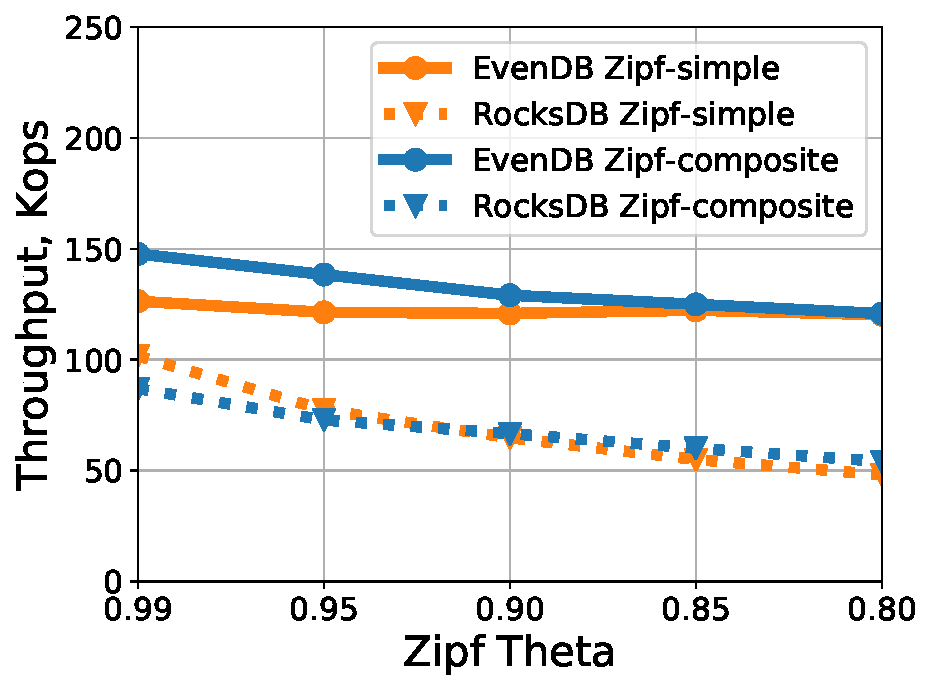
\includegraphics[width=\textwidth]{figs/puts_only_skew_line.pdf}
		\caption{\DIFaddFL{Put only}}
		\label{fig:puts_only_skew}
	\end{subfigure}
	\begin{subfigure}{0.48\linewidth}
		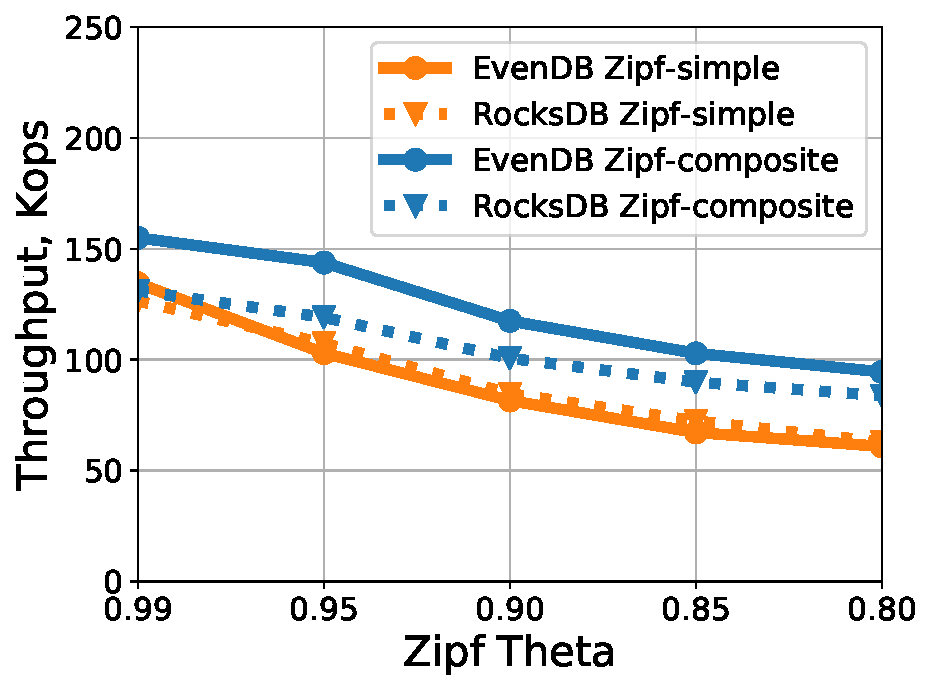
\includegraphics[width=\textwidth]{figs/gets_only_skew_line.pdf}
		\caption{\DIFaddFL{Get only}}
		\label{fig:gets_only_skew}
	\end{subfigure}
	\caption{{\DIFaddFL{The impact of the Zipf distribution's $\theta$ parameter (skew) on throughput, 64GB dataset.}}}
	\label{fig:skew_impact}
\end{figure}


\begin{table}
\begin{center}
\begin{tabular}{rccccc}
\DIFaddFL{$\theta=$	}& \DIFaddFL{0.99 }& \DIFaddFL{0.95 }& \DIFaddFL{0.90 }& \DIFaddFL{0.85 }& \DIFaddFL{0.80 }\\ 
	\hline 
	\DIFaddFL{Zipf-simple }& \DIFaddFL{4.87 }& \DIFaddFL{3.30 }& \DIFaddFL{1.91 }& \DIFaddFL{1.04 }& \DIFaddFL{0.54 }\\ 
	\DIFaddFL{Zipf-composite }& \DIFaddFL{0.013 }& \DIFaddFL{0.012 }& \DIFaddFL{0.010 }& \DIFaddFL{0.009 }& \DIFaddFL{0.008 }\\ 
\end{tabular} 
\end{center}
\caption{\DIFaddFL{Frequency ($\%$ of occurrences) of the most popular key under different $\theta$ values used for Zipf key generation.}}
\label{table:theta}
\end{table} 

\DIFaddend \subsection{Additional KV-Stores}
\label{ssec:pebbles} 

We experimented with Percona TokuDB~\cite{TokuDBgit}; although deprecated, no newer version is available. 
The results were at least an order-of-magnitude slower than RocksDB across the board, and therefore we do not present them. 
Note that this is in line with previously published comparisons~\cite{DBLP:conf/cidr/DongCGBSS17,tucana,toku-rocks-inno}.
We did not compare \sys\/  against
% the MySQL default KV-store, 
InnoDB because the latter is not easily separable 
from the MySQL code. Yet previous evaluations have found  InnoDB to be inferior to both RocksDB and TokuDB under 
write-abundant workloads~\cite{toku-rocks-inno}.

We next compare \sys\ to PebblesDB, which was shown to significantly improve over RocksDB~\cite{PebblesDB},
mostly in single-thread experiments, before RocksDB's recent version was released.  
We compare \sys\ to PebblesDB in a challenging  scenario for \sys, with a 32GB dataset and the Zipf-simple key 
distribution. We run each YCSB workload with 1, 2, 4, 8 and 12 threads. The results are summarized in Table~\ref{fig:pebbels-throughput}. 
While PebblesDB is slightly faster on some single-threaded benchmarks, from 2 threads and onward \sys\ is consistently better in all experiments, 
with an average performance improvement of almost \DIFdelbegin \DIFdel{1.8x}\DIFdelend \DIFaddbegin \DIFadd{$1.8\times$}\DIFaddend .  In all benchmarks, 
 \sys's advantage grows with the level of parallelism. We observed a similar trend with smaller datasets. 

We note that in our experiments, RocksDB also consistently outperforms PebblesDB. 
The discrepancy with the results reported in~\cite{PebblesDB} 
can be attributed, e.g., to RocksDB's evolution, resource constraints (running within a 
container), a different hardware setting, and increased  parallelism.   

\begin{table}
\centering
{\DIFdelbeginFL %DIFDELCMD < \small{
%DIFDELCMD < \begin{tabular}{cccccc}
%DIFDELCMD < %Workload & Zipf-simple & Zipf-composite \\
%DIFDELCMD < P & A & B, C & D& E10--1000 & F \\
%DIFDELCMD < \hline 
%DIFDELCMD < 0.86--2.8x & 0.94--1.6x & 1.4--2.3x &  0.98-2x & 1.0--3.4x &  0.84-1.23x  \\
%DIFDELCMD < \end{tabular}
%DIFDELCMD < }%%%
\DIFdelendFL \DIFaddbeginFL \small{
\begin{tabular}{cccccc}
%Workload & Zipf-simple & Zipf-composite \\
P & A & B, C & D& E10--1000 & F \\
\hline 
$0.9$--$2.8\times$ & $0.9$--$1.6\times$ & $1.4$--$2.3\times$ &  $1$--$2\times$ & $1$--$3.4\times$ &  $0.8$--$1.2\times$  \\
\end{tabular}
}\DIFaddendFL }
\caption{{\sys\/ throughput improvement over PebblesDB, 32GB dataset, Zipf-simple keys, 1--12 worker threads.
\sys's advantage grows with the number of threads.}}
\label{fig:pebbels-throughput}
\end{table}


\subsection{Insights}
\label{ssec:drill} 

\DIFaddbegin \paragraph{\DIFadd{Vertical scalability.}} 
\DIFadd{Figure~\ref{fig:scalability} illustrates \sys's throughput scaling for the 64GB dataset under Zipf-composite and Zipf-simple  
distributions. We exercise the A, C and P scenarios, with 1 to 12 worker threads.  
As expected, in C (100\% gets) \sys\/ scales nearly perfectly ($7.7\times$ for composite keys, $7.8\times$ for simple ones). 
The other workloads scale slower, due to read-write and write-write contention as well as background munk and funk rebalances. 
}


\begin{figure}[th]
\centering
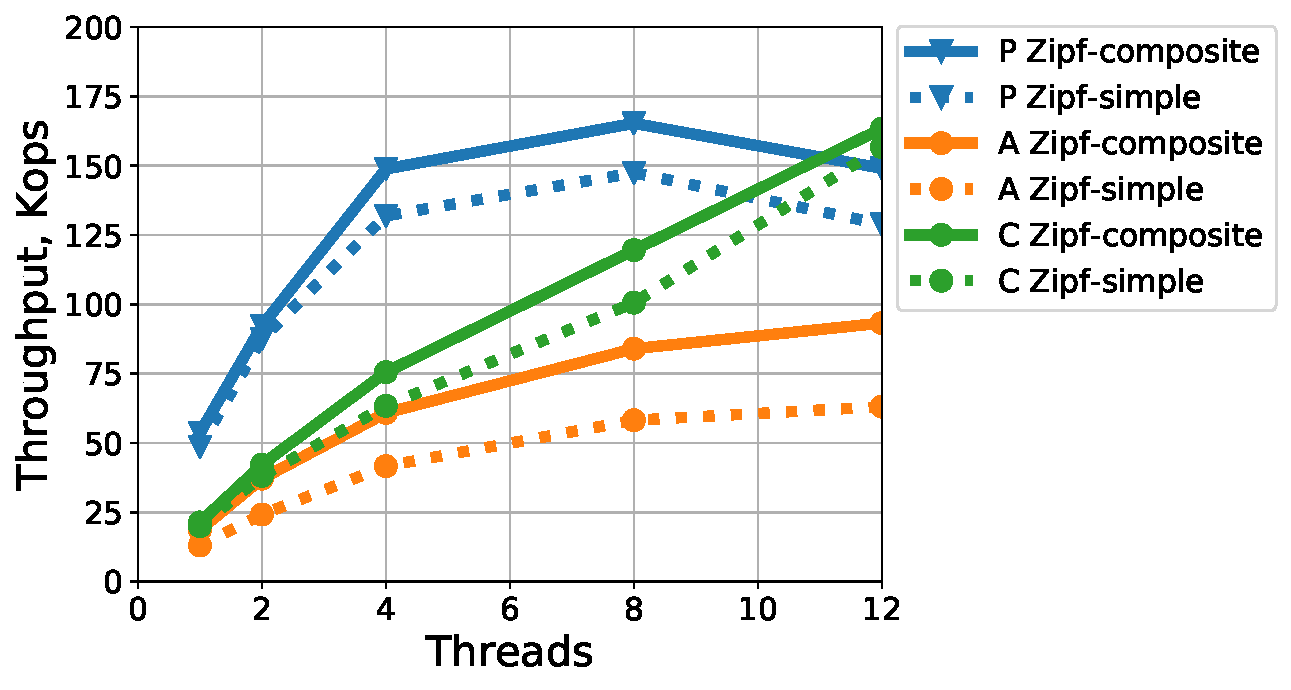
\includegraphics[width=0.4\textwidth]{figs/scalability_line.pdf}

\caption{{\DIFaddFL{\sys\/ scalability with the number of threads for 
the 64GB dataset and different workloads. }}}
\label{fig:scalability}
\end{figure}

\begin{figure}[htb]
\centering
\begin{subfigure}{0.48\linewidth}
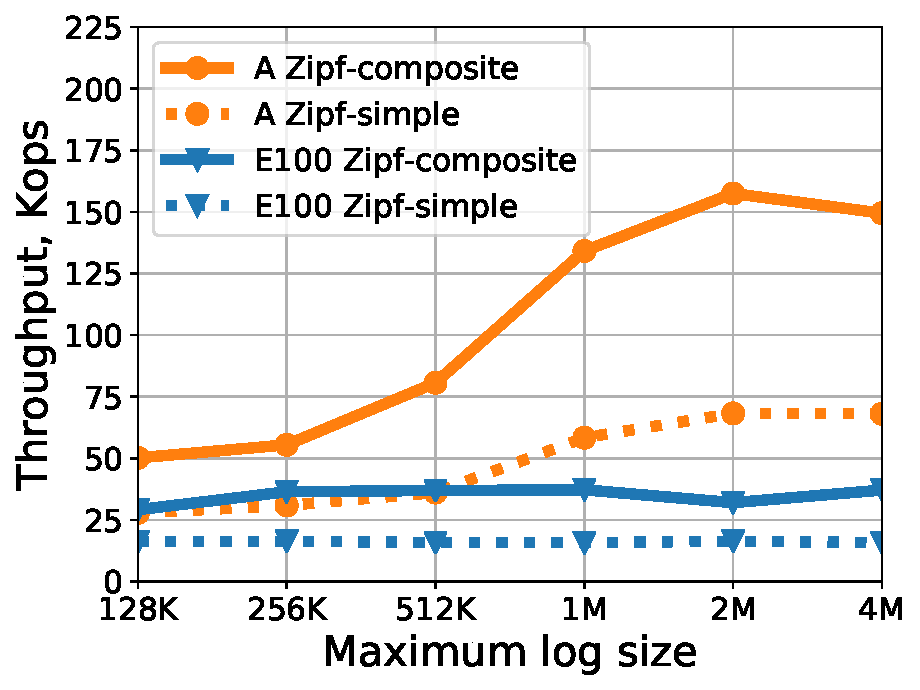
\includegraphics[width=\textwidth]{figs/max_log_size_line.pdf}
\caption{\DIFaddFL{Maximum log size,}\\  \DIFaddFL{workloads A and E100}}
\label{fig:params:log}
\end{subfigure}
\begin{subfigure}{0.48\linewidth}
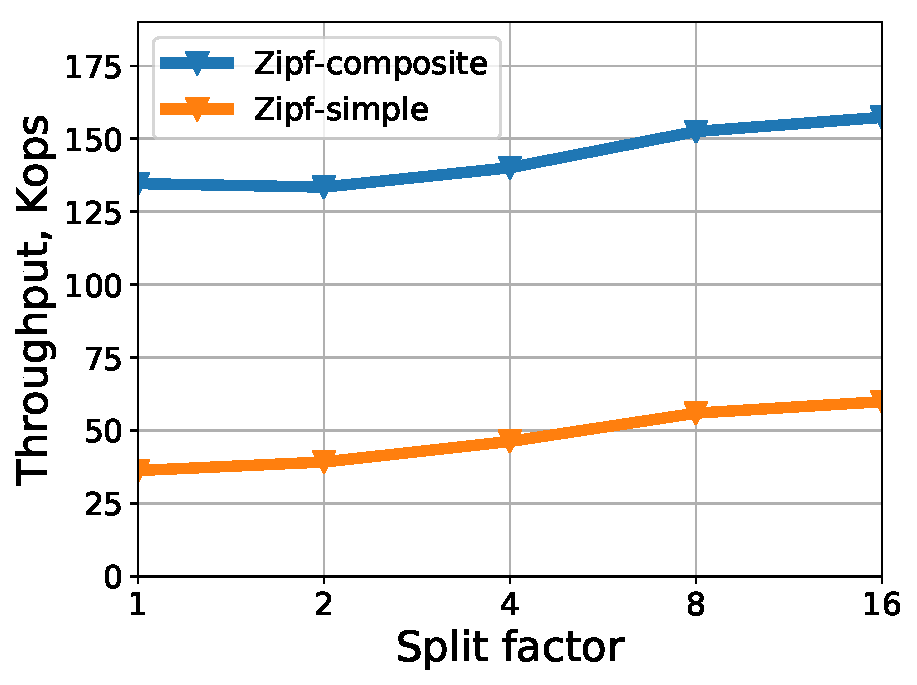
\includegraphics[width=\textwidth]{figs/Bloom_filter_line.pdf}
\caption{\DIFaddFL{Bloom filter split factor,}\\ \DIFaddFL{workload A}}
\label{fig:params:bf}
\end{subfigure}
\caption{{\DIFaddFL{\sys\/ throughput sensitivity to configuration parameters, on the 64GB dataset under  A (mixed put-get) and 
E100 (scan-dominant, 1 to 100 items).}}}
\label{fig:params}
\end{figure}

\paragraph{\DIFadd{\sys\/ configuration parameters.}} 
\DIFadd{We explore the system's  sensitivity to funk-log configuration parameters, for the most challenging 64GB dataset, 
and explain the choice of the default values.
}

\DIFadd{Figure~\ref{fig:params:log} depicts the throughput's dependency on the log size limit of munk-less funks, 
under  A and E100  with the Zipf-composite key distribution. 
The fraction of puts in A is 50\% (vs 5\% in E), which makes it more sensitive to the log size. 
A low threshold (e.g., 128KB) causes frequent funk rebalances, which degrades performance more than 3-fold. 
On the other hand, too high a threshold (4MB) lets the logs grow bigger, and slows down gets. Our experiments  
use 2MB logs, which favors write-intensive workloads. E favors smaller logs, since the write 
rate is low, and more funk rebalances can be accommodated. Its throughput can  grow by up to 20\% 
by tuning the system to use 512KB logs.
}

\DIFadd{Figure~\ref{fig:params:bf} depicts the throughput dependency on the Bloom filter split factor (i.e., the 
number of Bloom filters that summarize separate portions of the funk log) in workload A. 
Partitioning to 16 mini-filters gives the best result. %DIF > ; \inred{Idit: the following was not shown: beyond this point the benefit levels off}. 
The impact of Bloom filter partitioning on \sys's %DIF > end-to-end get latency as well as the 
memory footprint is negligible.
}

\paragraph{\DIFadd{RocksDB configuration tuning.}} \DIFadd{In RocksDB's out-of-the-box default configuration, the block cache is 8MB. 
We further experimented with block cache sizes of 1GB, 2GB, 5GB, and 8GB. We note that 
RocksDB's performance manual recommends allocating 1/3 of the available RAM 
($\sim$5GB) to the block cache~\mbox{%DIFAUXCMD
\cite{RocksDBMemoryTuning}}\hspace{0pt}%DIFAUXCMD
.
The results are mixed. For a small 
dataset (4GB) with composite keys, the block cache effectively replaces 
the OS pagecache, and improves RocksDB's throughput by $1.3\times$ and $1.6\times$
for workloads C and E100, respectively, by forgoing the system call overhead. This only partly reduces the gap between
RocksDB and \sys\/ in this setting. 
However, for  bigger datasets (32GB and 64GB),   using a  bigger block cache degrades  RocksDB's performance. 
%DIF > Figure~\ref{fig:rocks-memory} shows  RocksDB's speedup with different block cache sizes for the 64GB dataset in the various workloads. 
We found that the default configuration gives the best results for most of the workload suite. 
%DIF > (i.e., the  speedups are mostly below $1$). 
We therefore used this configuration  in~\S\ref{ssec:synthetic} above.   
}








\DIFaddend \section{Related Work}
\label{sec:related}


%common LSM stores RocksDB, scylladb, HyperLevelDB, LevelDB, hbase, cassandra
The vast majority of industrial mainstream NoSQL KV-stores are  implemented as LSM trees~\cite{hbase, 
RocksDB, scylladb, Bigtable2008, cassandra2010}, building on the foundations set by O'Neil 
et al.~\cite{DBLP:journals/acta/ONeilCGO96, Muth1998}. 

Due to LSM's design popularity, much effort has been invested into working around its bottlenecks.
A variety of compaction strategies has been implemented in production systems~\cite{CallaghanCompaction, 
ScyllaCompaction} and research prototypes~\cite{triad, PebblesDB, vttrees, slmdb}.  Improvements
 include storage
optimizations~\cite{WiscKey, PebblesDB, vttrees, slmdb,Papagiannis:2018:EMK:3267809.3267824}, 
boosting  in-memory parallelism~\cite{scylladb, clsm2015}, and leveraging 
 workload redundancies to defer disk flushes~\cite{triad, accordion} or avoid re-writing sorted data~\cite{vttrees}. 
In contrast to these, \sys\/ eliminates the concept of temporally-organized levels altogether
and employs a flat  layout with in-memory compaction.

\remove{
A number of systems focus on reducing write amplification.
PebblesDB~\cite{PebblesDB} introduces fragmented LSM trees in which level files are 
sliced into {\em guards\/} of increasing granularity and organized in a skiplist-like layout. 
%This structure reduces write amplification. 
In contrast, \sys\/ eliminates the concept of levels altogether, 
and employs a flat  layout. WiscKey~\cite{WiscKey} separates key and value storage 
in SSTables, also in order to reduce amplification. This optimization is orthogonal to \sys's concepts,
and could benefit our work as well. 
%
VT-Trees~\cite{vttrees} apply stitching to avoid rewriting already sorted data. This improves performance and significantly reduces write amplification in some scenarios (e.g., time-series ingestion).
}

SLM-DB~\cite{slmdb} is an LSM design that relies on persistent memory and thus eliminates the need for a WAL. It  
%re-designs the traditional LSM read path, 
utilizes a B$^+$-tree index in persistent memory on top of a flat list of temporally-partitioned SSTables. 
In contrast, \sys\ does not rely on special hardware. 
Moreover, to the best of our knowledge, SLM-DB does not support concurrent operations.

In-memory compaction has been recently implemented in HBase~\cite{accordion} by organizing
HBase's in-memory write store  as an LSM tree, eliminating redundancies 
in RAM to reduce disk flushes. However, being incremental to the LSM design, 
this approach fails to address spatial locality. 

Range-based  partitioning is also employed in  B-trees~\cite{Knuth:1998:ACP:280635} and their variants~\cite{Brodal:2003:LBE:644108.644201}. In
 \cref{ssec:B-tree-compare} we discussed the key challenges faced by storage systems adopting these designs, which 
 result in performance disadvantages compared to the LSM approach  (as shown, e.g., in~\cite{toku-rocks-inno}), 
 and the difficulty to support consistency  -- in particular, atomic scans --   under multi-threaded access.
 In contrast to B-tree nodes, \sys's chunks are not merely  a means to organize data on-disk; they 
are also the basic units for DRAM caching, I/O-batching, logging, and compaction. 
This allows us to apply chunk-level logging with sequential I/O and in-memory compaction.

 \remove{
 , which suffer from a write bottleneck in random updates to 
leaf blocks. \sys\/ overcomes this limitation through (1) transforming random I/O to sequential I/O at the chunk level, 
(2) managing a write-through chunk cache in memory (munks), and (3) reducing I/O  through in-memory (munk) compaction. 

A $B^{\epsilon}$-tree~\cite{Brodal:2003:LBE:644108.644201} is a B-tree variant that uses overflow write buffers in internal nodes. 
This design speeds up writes and reduces write amplification, however lookups are slowed down by having to search in unordered 
buffers. $B^{\epsilon}$-trees have been used in KV-stores (TokuDB~\cite{TokuDB}) and filesystems (BetrFS~\cite{BetrFS}).  
}

Tucana~\cite{tucana} is an in-memory $B^{\epsilon}$-tree index over a persistent log of KV-pairs. To speed up I/O, it
applies  system optimizations that are largely orthogonal to our work: block-device  access, copy-on-write on internal nodes, etc. However, Tucana provides neither strong scan semantics nor consistent recovery, and does not support concurrent puts.

A different line of work develops fast
in-memory (volatile) KV-stores~\cite{ignite, redis, memcached, Srinivasan:2016:AAR:3007263.3007276}, 
e.g., for web and application caches. Over time, many evolved to support durability,
yet still require the complete data set to reside in memory.
%For example, Ignite~\cite{ignite} uses a B-tree index with in-place random updates. 
%These systems resemble \sys\/ in their memory-centric approach. 
Although \sys\ is optimized for ``sliding-local'' scenarios where most of the active working set is in memory at any given time, it does not expect \emph{all} the data to fit in memory. 

Finally, \sys's in-munk data management leverages techniques used in concurrent in-memory KV-maps, e.g., partially-sorted 
key lists~\cite{Wu:2019:WFO:3302424.3303955,kiwi}, lazy index updates~\cite{kiwi,tdls}, 
and synchronizing scans with puts via a PO array~\cite{kiwi}. These aspects are important, but since they do not involve I/O, they do not have a major impact on overall performance.

%Their persistent storage support is based on either B-tree~\cite{ignite} or LSM-tree design~\cite{redis}. 
%used for application data caching, but also as building blocks for distributed database with optional durability~\cite{ignite,redis}. These are not comparable with \sys\ as they are either not persistent~\cite{memcached}, do not support atomic scans~\cite{redis} or resemble  relational DBMS with a centralized WAL, , and in-place updates~\cite{ignite}  more than a KV LSM store.

\section{Conclusions}
\label{sec:conclusions}
We presented \sys\/ -- a novel persistent KV-store optimized for workloads with high spatial locality, as prevalent in modern %data-driven 
applications. \sys\/ provides strong (atomic) consistency guarantees for random updates, random lookups, and range queries. 
\sys\/ outperforms the state-of-the-art RocksDB LSM store  in the  majority of YCSB benchmarks, with both 
standard and spatially-local key distributions, in which it excels in particular. \sys\/ further reduces write amplification to near-optimal under write-intensive 
workloads. Finally, it provides near-instant recovery from failures.
%, in contrast to traditional data stores based on centralized write-ahead logs.

Beyond building a particular system prototype, this paper puts forth a novel KV-store design alternative that emphasizes spatial locality. We hope to see future realizations of this approach with various improvements, through novel ideas or ones borrowed from other existing solutions. 
%It can also benefit from new hardware trends, in particular, non-volatile memory technologies.  

\bibliographystyle{acm}
 %\bibliography{ref}

\clearpage
%{\normalsize \bibliographystyle{acm}
\begin{thebibliography}{10}

\bibitem{RocksDBMemoryTuning}
https://github.com/facebook/rocksdb/wiki/Setup-Options-and-Basic-Tuning\#block-cache-size.

\bibitem{appsflyer}
Appsflyer.
\newblock \url{https://appsflyer.com}.

\bibitem{flurry}
Flurry analytics.
\newblock \url{https://flurry.com}.

\bibitem{FlurryReport2017}
Flurry state of the mobile 2018.
\newblock
  \url{https://www.verizonmedia.com/insights/flurry-analytics-releases-2017-state-of-mobile-report}.

\bibitem{firebase}
Google firebase.
\newblock \url{https://firebase.google.com}.

\bibitem{ignite}
{Ignite } database and caching platform.
\newblock {https://ignite.apache.org/}.

\bibitem{innodblocking}
Innodblocking.
\newblock \url{https://dev.mysql.com/doc/refman/8.0/en/innodb-locking.html}.

\bibitem{alliedmarketresearch}
{NoSQL} market is expected to reach \$4.2 billion, globally, by 2020.
\newblock
  {https://www.alliedmarketresearch.com/press-release/NoSQL-market-is-expected-to-reach-4-2-billion-globally-by-2020-allied-market-research.html}.

\bibitem{redis}
Redis, an open source, in-memory data structure store.
\newblock {https://redis.io/}.

\bibitem{rocksdb-benchmarks}
{RocksDB} performance benchmarks.
\newblock {https://github.com/facebook/rocksdb/wiki/performance-benchmarks}.

\bibitem{RocksDBPerf}
{RocksDB} tuning guide.
\newblock {https://github.com/facebook/rocksdb/wiki/RocksDB-Tuning-Guidel}.

\bibitem{hbase}
Apache hbase, a distributed, scalable, big data store.
\newblock \url{http://hbase.apache.org/}, Apr. 2014.

\bibitem{leveldb}
A fast and lightweight key/value database library by google.
\newblock \url{http://code.google.com/p/leveldb}, Jan. 2014.

\bibitem{RocksDB}
A persistent key-value store for fast storage environments.
\newblock \url{http://rocksdb.org/}, June 2014.

\bibitem{Cpp-YCSB}
{Yahoo! Cloud Serving Benchmark in C++, a C++ version of YCSB}.
\newblock \url{https://github.com/basicthinker/YCSB-C}, 2014.

\DIFdelbegin %DIFDELCMD < \bibitem{dram-prices}
%DIFDELCMD < {%%%
\DIFdel{Average selling price of DRAM 1Gb equivalent units from 2009 to 2017 (in U.S.
  dollars)}%DIFDELCMD < }%%%
\DIFdel{.
}%DIFDELCMD < \newblock
%DIFDELCMD <   \url{https://www.statista.com/statistics/298821/dram-average-unit-price/}%%%
\DIFdel{,
  2018.
}%DIFDELCMD < 

%DIFDELCMD < %%%
\DIFdelend \bibitem{memcached}
Memcached, an open source, high-performance, distributed memory object caching
  system.
\newblock \url{https://memcached.org/}, Dec. 2018.

\bibitem{TokuDB}
{Percona TokuDB}.
\newblock \url{https://www.percona.com/software/mysql-database/percona-tokudb},
  2018.

\bibitem{scylladb}
Scylla the real-time big data database.
\newblock \url{https://www.scylladb.com/}, 2018.

\bibitem{pebbles-git-issue}
Versionset::removefilelevelbloomfilterinfo isn't thread-safe.
\newblock https://github.com/utsaslab/pebblesdb/issues/19, January 2018.

\bibitem{TokuDBgit}
{PerconaFT is a high-performance, transactional key-value store}.
\newblock \url{https://github.com/percona/PerconaFT}, 2019.

\bibitem{Armstrong:2013:LDB:2463676.2465296}
{\sc Armstrong, T.~G., Ponnekanti, V., Borthakur, D., and Callaghan, M.}
\newblock Linkbench: A database benchmark based on the facebook social graph.
\newblock In {\em Proceedings of the 2013 ACM SIGMOD International Conference
  on Management of Data\/} (New York, NY, USA, 2013), SIGMOD '13, ACM,
  pp.~1185--1196.

\bibitem{triad}
{\sc Balmau, O., Didona, D., Guerraoui, R., Zwaenepoel, W., Yuan, H., Arora,
  A., Gupta, K., and Konka, P.}
\newblock Triad: Creating synergies between memory, disk and log in log
  structured key-value stores.
\newblock In {\em Proceedings of the 2017 USENIX Conference on Usenix Annual
  Technical Conference\/} (2017), USENIX ATC '17, pp.~363--375.

\bibitem{kiwi}
{\sc Basin, D., Bortnikov, E., Braginsky, A., Golan-Gueta, G., Hillel, E.,
  Keidar, I., and Sulamy, M.}
\newblock Kiwi: A key-value map for scalable real-time analytics.
\newblock In {\em Proceedings of the 22Nd ACM SIGPLAN Symposium on Principles
  and Practice of Parallel Programming\/} (2017), PPoPP '17, ACM, pp.~357--369.

\bibitem{Borthakur:2011:AHG:1989323.1989438}
{\sc Borthakur, D., Gray, J., Sarma, J.~S., Muthukkaruppan, K., Spiegelberg,
  N., Kuang, H., Ranganathan, K., Molkov, D., Menon, A., Rash, S., Schmidt, R.,
  and Aiyer, A.}
\newblock Apache hadoop goes realtime at facebook.
\newblock In {\em Proceedings of the 2011 ACM SIGMOD International Conference
  on Management of Data\/} (2011), SIGMOD '11, pp.~1071--1080.

\bibitem{accordion}
{\sc Bortnikov, E., Braginsky, A., Hillel, E., Keidar, I., and Sheffi, G.}
\newblock Accordion: Better memory organization for lsm key-value stores.
\newblock {\em Proc. VLDB Endow. 11}, 12 (Aug. 2018), 1863--1875.

\bibitem{Brodal:2003:LBE:644108.644201}
{\sc Brodal, G.~S., and Fagerberg, R.}
\newblock Lower bounds for external memory dictionaries.
\newblock In {\em Proceedings of the Fourteenth Annual ACM-SIAM Symposium on
  Discrete Algorithms\/} (2003), SODA '03, pp.~546--554.

\bibitem{CallaghanCompaction}
{\sc Callaghan, M.}
\newblock {Name that compaction algorithm}.
\newblock
  \url{https://smalldatum.blogspot.com/2018/08/name-that-compaction-algorithm.html},
  2018.
\DIFaddbegin 

\bibitem{facebook-workloads}
{\sc \DIFadd{Cao, Z., Dong, S., Vemuri, S., and Du, D.~H.}}
\newblock \DIFadd{Characterizing, modeling, and benchmarking }{\DIFadd{RocksDB}} \DIFadd{key-value
  workloads at }{\DIFadd{Facebook}}\DIFadd{.
}\newblock \DIFadd{In }{\em \DIFadd{USENIX Conference on File and Storage Technologies (FAST)\/}}
  \DIFadd{(2020).
}\DIFaddend 

\bibitem{Bigtable2008}
{\sc Chang, F., Dean, J., Ghemawat, S., Hsieh, W.~C., Wallach, D.~A., Burrows,
  M., Chandra, T., Fikes, A., and Gruber, R.~E.}
\newblock Bigtable: A distributed storage system for structured data.
\newblock {\em ACM Trans. Comput. Syst. 26}, 2 (June 2008), 4:1--4:26.

\bibitem{Cho:1998:ECT:297805.297835}
{\sc Cho, J., Garcia-Molina, H., and Page, L.}
\newblock Efficient crawling through url ordering.
\newblock In {\em Proceedings of the Seventh International Conference on World
  Wide Web 7\/} (1998), WWW7, pp.~161--172.

\bibitem{YCSB}
{\sc Cooper, B.~F., Silberstein, A., Tam, E., Ramakrishnan, R., and Sears, R.}
\newblock Benchmarking cloud serving systems with ycsb.
\newblock In {\em Proceedings of the 1st ACM Symposium on Cloud Computing\/}
  (2010), SoCC '10, pp.~143--154.

\bibitem{DBLP:conf/cidr/DongCGBSS17}
{\sc Dong, S., Callaghan, M., Galanis, L., Borthakur, D., Savor, T., and Strum,
  M.}
\newblock Optimizing space amplification in rocksdb.
\newblock In {\em {CIDR} 2017, 8th Biennial Conference on Innovative Data
  Systems Research, Chaminade, CA, USA, January 8-11, 2017, Online
  Proceedings\/} (2017), www.cidrdb.org.

\bibitem{tinyLFU}
{\sc Einziger, G., Friedman, R., and Manes, B.}
\newblock Tinylfu: A highly efficient cache admission policy.
\newblock {\em ACM Trans. Storage 13}, 4 (Nov. 2017), 35:1--35:31.

\bibitem{clsm2015}
{\sc Golan-Gueta, G., Bortnikov, E., Hillel, E., and Keidar, I.}
\newblock Scaling concurrent log-structured data stores.
\newblock In {\em {EuroSys}\/} (2015), pp.~32:1--32:14.

\bibitem{toku-rocks-inno}
{\sc Iyer, S.}
\newblock Comparing tokudb, rocksdb and innodb performance on intel(r) xeon(r)
  gold 6140 cpu.
\newblock
  https://minervadb.com/index.php/2018/08/06/comparing-tokudb-rocksdb-and-innodb-performance-on-intelr-xeonr-gold-6140-cpu/,
  2018.

\bibitem{slmdb}
{\sc Kaiyrakhmet, O., Lee, S., Nam, B., Noh, S.~H., and ri~Choi, Y.}
\newblock {SLM-DB}: Single-level key-value store with persistent memory.
\newblock In {\em 17th {USENIX} Conference on File and Storage Technologies
  ({FAST} 19)\/} (2019), pp.~191--205.

\bibitem{Knuth:1998:ACP:280635}
{\sc Knuth, D.~E.}
\newblock {\em The Art of Computer Programming, Volume 3: (2Nd Ed.) Sorting and
  Searching}.
\newblock Addison Wesley Longman Publishing Co., Inc., Redwood City, CA, USA,
  1998.

\bibitem{cassandra2010}
{\sc Lakshman, A., and Malik, P.}
\newblock Cassandra: A decentralized structured storage system.
\newblock {\em SIGOPS Oper. Syst. Rev. 44}, 2 (Apr. 2010), 35--40.

\bibitem{WiscKey}
{\sc Lu, L., Pillai, T.~S., Gopalakrishnan, H., Arpaci-Dusseau, A.~C., and
  Arpaci-Dusseau, R.~H.}
\newblock Wisckey: Separating keys from values in ssd-conscious storage.
\newblock {\em ACM Trans. Storage 13}, 1 (Mar. 2017), 5:1--5:28.

\bibitem{rocks-vs-inno}
{\sc Matsunobu, Y.}
\newblock Myrocks: A space- and write-optimized mysql database.
\newblock
  \url{https://engineering.fb.com/core-data/myrocks-a-space-and-write-optimized-mysql-database/},
  2016.

\bibitem{Muth1998}
{\sc Muth, P., O'Neil, P.~E., Pick, A., and Weikum, G.}
\newblock Design, implementation, and performance of the lham log-structured
  history data access method.
\newblock In {\em Proceedings of the 24rd International Conference on Very
  Large Data Bases\/} (1998), VLDB '98, pp.~452--463.

\bibitem{DBLP:journals/acta/ONeilCGO96}
{\sc O'Neil, P.~E., Cheng, E., Gawlick, D., and O'Neil, E.~J.}
\newblock The log-structured merge-tree (lsm-tree).
\newblock {\em Acta Inf. 33}, 4 (1996), 351--385.

\bibitem{tucana}
{\sc Papagiannis, A., Saloustros, G., Gonz\'{a}lez-F{\'e}rez, P., and Bilas,
  A.}
\newblock Tucana: Design and implementation of a fast and efficient scale-up
  key-value store.
\newblock In {\em Proceedings of the 2016 USENIX Conference on Usenix Annual
  Technical Conference\/} (2016), USENIX ATC '16, pp.~537--550.

\bibitem{Papagiannis:2018:EMK:3267809.3267824}
{\sc Papagiannis, A., Saloustros, G., Gonz\'{a}lez-F{\'e}rez, P., and Bilas,
  A.}
\newblock An efficient memory-mapped key-value store for flash storage.
\newblock In {\em Proceedings of the ACM Symposium on Cloud Computing\/} (New
  York, NY, USA, 2018), SoCC '18, ACM, pp.~490--502.

\bibitem{PebblesDB}
{\sc Raju, P., Kadekodi, R., Chidambaram, V., and Abraham, I.}
\newblock Pebblesdb: Building key-value stores using fragmented log-structured
  merge trees.
\newblock In {\em Proceedings of the 26th Symposium on Operating Systems
  Principles\/} (2017), SOSP '17, pp.~497--514.

\bibitem{vttrees}
{\sc Shetty, P.~J., Spillane, R.~P., Malpani, R.~R., Andrews, B., Seyster, J.,
  and Zadok, E.}
\newblock Building workload-independent storage with vt-trees.
\newblock In {\em Presented as part of the 11th {USENIX} Conference on File and
  Storage Technologies ({FAST} 13)\/} (2013), pp.~17--30.

\bibitem{tdls}
{\sc Spiegelman, A., Golan-Gueta, G., and Keidar, I.}
\newblock Transactional data structure libraries.
\newblock In {\em Proceedings of the 37th ACM SIGPLAN Conference on Programming
  Language Design and Implementation\/} (2016), PLDI '16, pp.~682--696.

\bibitem{Srinivasan:2016:AAR:3007263.3007276}
{\sc Srinivasan, V., Bulkowski, B., Chu, W.-L., Sayyaparaju, S., Gooding, A.,
  Iyer, R., Shinde, A., and Lopatic, T.}
\newblock Aerospike: Architecture of a real-time operational dbms.
\newblock {\em Proc. VLDB Endow. 9}, 13 (Sept. 2016), 1389--1400.

\bibitem{ScyllaCompaction}
{\sc Tribble, P.}
\newblock {How to Ruin Your Performance by Choosing the Wrong Compaction
  Strategy}.
\newblock
  \url{https://www.scylladb.com/2017/12/28/compaction-strategy-scylla/}, 2017.

\bibitem{Wu:2019:WFO:3302424.3303955}
{\sc Wu, X., Ni, F., and Jiang, S.}
\newblock Wormhole: A fast ordered index for in-memory data management.
\newblock In {\em Proceedings of the Fourteenth EuroSys Conference 2019\/} (New
  York, NY, USA, 2019), EuroSys '19, ACM, pp.~18:1--18:16.

\end{thebibliography}

%}

%\theendnotes

\end{document}
